%%% Exemplo de utilização da classe ITA
%%%
%%%   por        Fábio Fagundes Silveira   -  ffs [at] ita [dot] br
%%%              Benedito C. O. Maciel     -  bcmaciel [at] ita [dot] br
%%%              Giovani Volnei Meinertz   -  giovani [at] ita [dot] br
%%%    	         Hudson Alberto Bode       -  bode [at] ita [dot]br
%%%    	         P. I. Braga de Queiroz    -  pi [at] ita [dot] br
%%%    	         Jorge A. B. Gripp         -  gripp [at] ita [dot] br
%%%    	         Juliano Monte-Mor         -  jamontemor [at] yahoo [dot] com [dot] br
%%%    	         Tarcisio A. B. Gripp      -  tarcisio.gripp [at] gmail [dot] com
%%%    	         
%%%
%%%  IMPORTANTE: O texto contido neste exemplo nao significa absolutamente nada.  :-)
%%%              O intuito aqui eh demonstrar os comandos criados na classe e suas
%%%              respectivas utilizacoes.
%%%
%%%  Tese.tex  2016-08-25
%%%  $HeadURL: http://www.apgita.org.br/apgita/teses-e-latex.php $
%%%
%%% ITALUS
%%% Instituto Tecnológico de Aeronáutica --- ITA, Sao Jose dos Campos, Brasil
%%%                   http://groups.yahoo.com/group/italus/
%%% Discussion list: italus {at} yahoogroups.com
%%%
%++++++++++++++++++++++++++++++++++++++++++++++++++++++++++++++++++++++++++++++
% Para alterar o TIPO DE DOCUMENTO, preencher a linha abaixo \documentclass[?]{?}
%   \documentclass[tg]{ita}			= Trabalho de Graduacao
%   \documentclass[tgfem]{ita}		= Para Engenheiras
%   								msc     		= Dissertacao de Mestrado
%   								mscfem   		= Para Mestras
%   								dsc      		= Tese de Doutorado
%   								dscfem   		= Para Doutoras
%   								quali    		= Exame de Qualificacao
%   								qualifem 		= Exame de Qualificacao para Doutoras
% Para 'Draft Version'/'Versao Preliminar' com data no rodape, adicionar 'dv':
%   \documentclass[dsc, dv]{ita} 
% Para trabalhos em Inglês, adicionar 'eng':
%   \documentclass[dsc, eng]{ita}
%		\documentclass[dsc, eng, dv]{ita}
%++++++++++++++++++++++++++++++++++++++++++++++++++++++++++++++++++++++++++++++
\documentclass[tg, eng]{ita}    % ITA.cls based on standard book.cls 
% Quando alterar a classe, por exemplo de [msc] para [msc, eng]) rode mais uma vez o botão BUILD OUTPUT caso haja erro
\usepackage{booktabs}
\usepackage{ae}
\usepackage{subcaption}
\usepackage{graphicx}
\usepackage{epsfig}
\usepackage{amsmath}
\usepackage{amssymb} 
%\usepackage{subfig}
\usepackage{multirow}
\usepackage{float}
\usepackage{lipsum}
\usepackage{longtable}
\usepackage{array}

\usepackage{algorithm} 
\usepackage{algpseudocode}

\algdef{SE}{Begin}{End}{\textbf{begin}}{\textbf{end}}

%++++++++++++++++++++++++++++++++++++++++++++++++++++++++++++++++++++++++++++++
% Espaçaamento padrão de todo o documento
%++++++++++++++++++++++++++++++++++++++++++++++++++++++++++++++++++++++++++++++
\onehalfspacing

%singlespacing Para um espaçamento simples
%onehalfspacing Para um espaçamento de 1,5
%doublespacing Para um espaaçamento duplo

%++++++++++++++++++++++++++++++++++++++++++++++++++++++++++++++++++++++++++++++
% Identificacoes (se o trabalho for em inglês, insira os dados em inglês)
% Para entradas abreviadas de Professora (Profa.) em português escreva: Prof$^\textnormal{a}$.
%++++++++++++++++++++++++++++++++++++++++++++++++++++++++++++++++++++++++++++++
\course{Computer Engineering} % Programa de PG ou Curso de Graduação
% \area{Sistemas Aeroespaciais e Mecatrônica} % área de concentração na PG (Não utilizado no caso de TG)

% Autor do trabalho: Nome Sobrenome
\authorgender{masc} %sexo: masc ou fem
\author{Heládio Sampaio}{Lopes}
\itaauthoraddress{H8A St., 113}{12228-460}{São José dos Campos--SP}

% Titulo da Tese/Dissertação
\title{Natural Language Processing for Trend Forecasting}

% Orientador
\advisorgender{masc} % masc ou fem
\advisor{Prof. Dr.}{Filipe Alves Neto Verri}{ITA}

% Coorientador (Caso no haja coorientador, colocar ambas as variveis \coadvisorgender e \coadvisor comentadas, com um % na frente)
% \coadvisorgender{fem}									% masc ou fem
% \coadvisor{~Dr$^\textnormal{a}$.}{Rosa de Fátima Cruz Marques}{IAE}

% Pró-reitor da Pós-graduação
% \bossgender{masc}												% masc ou fem
% \boss{Prof.~Dr.}{John von Neumann}

%Coordenador do curso no caso de TG
\bosscoursegender{masc}									% masc ou fem
\bosscourse{Prof.~Dr.}{Inaldo Capistrano Costa}

% Palavras-Chaves informadas pela Biblioteca -> utilizada na CIP
\kwcip{Natural Language Processing}
\kwcip{Topic Modeling}
\kwcip{Machine Learning}

% membros da banca examinadora

% \examiner{Prof. Dr.}{Alan Turing}{Presidente}{ITA}
% \examiner{Prof. Dr.}{Linus Torwald}{}{UXXX}
% \examiner{Prof. Dr.}{Richard Stallman}{}{UYYY}
% \examiner{Prof. Dr.}{Donald Duck}{}{DYSNEY}
% \examiner{Prof. Dr.}{Mickey Mouse}{}{DISNEY}

% Data da defesa (més em maiúsculo, se trabalho em inglês, e minusculo se trabalho em português) 
\date{20}{November}{2020}

% Número CDU - (somente para TG)
\cdu{621.38}

% Glossario
\makeglossary
\frontmatter

\begin{document}	
% Folha de Rosto e Capa para o caso do TG
\maketitle

% Dedicatoria: Nao esqueca essa secao  ... :-)
\begin{itadedication}
To my lovely mother, who has always supported me through this tough journey.
\end{itadedication}

% Agradecimentos
\begin{itathanks}
Thank you
\end{itathanks}

% Epígrafe
\thispagestyle{empty}
\ifhyperref\pdfbookmark[0]{\nameepigraphe}{epigrafe}\fi
\begin{flushright}
\begin{spacing}{1}
\mbox{}\vfill
{\sffamily\itshape
``Quanto mais difícil for a vitória, maior será sua felicidade em ganhar.''\\}
--- Pel\'e \textsc{}
\end{spacing}
\end{flushright}

% Resumo
\begin{abstract}
\noindent
Com avanço cientifico-tecnológico em escalas globais, a disponibilidade de dados para serem analisados cresce de maneira exponencial. A partir desse crescimento acelerado, técnicas de inteligência artificial, como o Processamento de Linguagem Natural (PLN), ajudam a automatizar o processo de se extrair informação de documentos.  Com intuito de realizar previsões sobre as tendências que surgirão em meio ao crescimento de dados, é possível utilizar técnicas de modelagem de tópicos para agrupar documentos em temas semelhantes e estudar a incidência temporal desses temas.

Assim, este trabalho busca aplicar técnicas de PLN combinadas com aprendizado supervisionado para agrupar documentos em um conjunto de temas e a partir disso aprender a identificá-los em novos documentos em um período futuro. Utilizando publicações cientificas da conferência de Sistemas de Processamento de Informação Neural, fomos capazes de modelar essa tarefa e obter bons resultados. Também estudamos a capacidade dos classificadores de manter desempenho satisfatório com o passar do tempo.

\end{abstract}

% Abstract
\begin{englishabstract}
\noindent
With scientific and technological advances on global scales, the availability of data to be analyzed grows exponentially. Based on this accelerated growth, artificial intelligence techniques, such as Natural Language Processing (NLP), increasingly help to automate the process of extracting information from documents. In order to make predictions about the trends that will arise from data growth, it is possible to use topic modeling techniques to group documents on similar clusters and study the temporal incidence of those topics.

Thereby, this work aims to apply NLP techniques combined with supervised learning to group documents into a set of themes and from there learn to identify them in new documents in a future period. Using scientific publications from the Conference on Neural Information Processing Systems, we were able to model this task and obtain good results, \dots
% TODO: terminar o texto para ficar coerente com a modificação no texto em português

\end{englishabstract}

% Lista de figuras
\listoffigures %opcional

% Lista de tabelas
\listoftables %opcional

% Lista de abreviaturas
\listofabbreviations
\begin{longtable}{ll}
	AI     & Artificial Intelligence                   \\
	BoW    & Bag of Words                              \\
	CBOW   & Continuous Bag of Words                   \\
	FN     & False Negative                            \\
	FP     & False Positive                            \\
	IT     & Information Technology                    \\
	LDA    & Latent Dirichelt Allocation               \\
	LOWESS & Locally Weighted Scatterplot Smoothing    \\
	ML     & Machine Learning                          \\
	NIPS   & Neural Information Processing Systems     \\
	NLP    & Natural Language Processing               \\
	NPMI   & Normalized Pointwise Mutual Information   \\
	OLS    & Ordinary Least Squares                    \\
	TF-IDF & Term Frequency Inverse Document Frequency \\
	TN     & True Negative                             \\
	TP     & True Positive                             \\
\end{longtable}

 %opcional

% Lista de simbolos
%\listofsymbols
%%\begin{longtable}{ll}
%$a$ & Distncia\\
%$\textbf{a}$ & Vetor de distncias\\
%$\textbf{e}_{j}$ & Vetor unitrio de dimenso $n$ e com o $j$-simo componente igual a $1$ \\
%$\textbf{K}$ & Matriz de rigidez\\
%$m_1$ & Massa do cumpim\\
%$\delta_{k-k_f}$ & Delta de Kronecker no instante $k_f$\\
%
%\end{longtable}
%
 %opcional

% Sumario
\tableofcontents

\mainmatter
% Os capitulos comecam aqui

\chapter{Introduction}\label{chap:intro}
Recently, the growth of artificial intelligence has been helping us to solve problems in most various areas, including linguistics. With natural language processing techniques, computers can process text in order to extract information faster than humans.

\section{Motivation}

%Every kind of expression, verbal or in writing, brings us much information to be interpreted. Whether the topic is chosen, the tone used, the choice of words, everything can be interpreted, and then generate some valuable information. Over the years, more and more knowledge is generated and we humans are unable to process such an amount of information. Natural Language Processing emerges as a technology capable of assisting us in this hard task.

%\citeonline{state_of_the_art} defines Natural Language Processing, abbreviated by NLP, as a branch of artificial intelligence capable of making computers comprehend and extract information from human language. NLP can perform a lot of tasks, such as identifying different topics for a set of documents, classifying texts on predefined subjects, and beyond that extract the sentiment to know what people are saying about something.

%The topic discovery was widely explored in the literature, \citeonline{hurtado2016topic} and \citeonline{jelodar2020deep} use it to group, respectively, papers abstracts and comments in social media in similar clusters. In a long period, it is possible to analyze how these founded topics behave through time and make predictions about the near future.

Every kind of expression, verbal or in writing, brings us much information to be interpreted. Whether the topic is chosen, the tone used, the choice of words, everything can be interpreted, and then generate some valuable information.

Over the years, more and more knowledge is generated and we humans are unable to process such an amount of information. A study made by \citeonline{beath2012finding} reveals that the enterprises' volume of data is expanding by 35\%-50\% every year, including textual data. Despite this, they also find that the companies could not extract information from this huge amount of data.

In that way, extracting valuable information from this data has become more and more an important skill. Therefore, Natural Language Processing emerges as a technology capable of assisting us in the task of deal with textual data.

\citeonline{khurana2017natural} defines Natural Language Processing, abbreviated by NLP, as a branch of artificial intelligence capable of making computers comprehend and extract information from human language.
In fact, NLP can perform simple tasks but not quite scalable for a human, such as translate text from one language to another, identify different topics for a set of documents, classify text on predefined subjects, and beyond that extract the sentiment to know what people are saying about something.

% Falar sobre alexa, google assistente e siri.
In recent years a particular kind of NLP application is drawing a lot of attention. The voice assistants like Siri, Cortana, Alexa and Google Assistant are the hot AI topics of the moment. Together, all digital assistants attempted to answer more and more questions each year, \cite{kailakrayewski2019}.

\newpage
In our particular scope, the topic discovery was widely explored in the literature. \citeonline{hurtado2016topic} and \citeonline{jelodar2020deep} use it to group, respectively, papers abstracts and comments in social media in similar clusters. The first one uses it to study the topics' evolution and correlation between the founded topics. In contrast, the second group comments to analyze the general sentiment about them.

However, these related works apply topic modeling only for static analysis. In this work context, we are seeking a real-time application that will keep receiving news in a continuous process. Thus, redo the topic discovery process will demand an expensive computational cost, besides the human effort to label the topics. To avoid the rework of modeling the documents in topics, a classification-based system will be proposed, for a future development of a real-time application is possible.


\section{Objective}

%Curious about the fast world's evolution, this work aims to implement Natural Language Processing techniques to propose a framework capable of modeling in real-time the topics' evolution over the years. With this in mind, evaluate the ability of those models to make predictions about future trends.

Curious about the fast world's evolution, this work aims to implement Natural Language Processing techniques to propose a framework capable of modeling in real-time the topics' evolution over time, using an annual granularity. 
With this in mind, we must evaluate the ability of those models in modeling the themes occurrence over the years.

By the end of this work, a series of tasks must be done. First, we must normalize the documents to segment them into time-ordered subsets, \textit{Past}, \textit{Present} and \textit{Future}, respectively. With the eldest subset, we must find meaningful subjects to train classification models based on these topics. Then, evaluate the predictions for \textit{Present} set and how the models' performance degenerates over the years.

% Esta seção deve conter:
%   - Objetivo geral: propor um framework para aprender evolução de tópicos em texto em
%     linguagem natural ao longo do tempo.
%   - Objetivos específicos:
%     a) Propor a divisão da base de dados em diferentes conjuntos
%     b) Encontrar os tópicos no passado
%     c) Treinar classificadores
%     d) Avaliar o desempenho no presente
%     e) Avaliar a degeneração do desempenho

%\section{Objective}
%
%As already discussed, we want to build models capable of making predictions regarding the evolution of discovered topics in a set of documents. We also want to find topics in real-time at each received document without having to redo the topic discovery process. Then, by the end of this work, we must have performed the tasks listed below.
%
%\begin{itemize}
%	\item Find a database long enough, over several years;
%	\item Perform all necessary treatment steps to normalize the documents' texts;
%	\item Find meaningful topics in a subset from the original database;
%	\item Create a topic classifier to find out if a document addresses any topic of interest;
%	\item Model topic evolution to evaluate the forecast accuracy.
%\end{itemize}

\section{Organization of this work}

The remaining of this work is organized as follows: Chapter \ref{chap:literature} will cover the theory behind Natural Language Processing and basics Classification. Chapter \ref{chap:related} will describe some previous works which use topic discovery and trend forecast. Chapter \ref{chap:materials} will better explain the problem and the methodology that will be used to handle it. Chapter \ref{chap:results} will show the discovered results for the proposed experiment and some discussion about them. Finally, Chapter \ref{chap:conclusion} will present some conclusions and suggestions for future work.


\chapter{Literature Review}\label{chap:literature}
In this chapter, we will introduce the general concepts and techniques behind Natural Language Processing. We will cover all the necessary steps for extracting meaningful topics from texts. Finally, a brief discussion about machine learning for tasks like classification and regression.


\section{Natural Language Processing}

	In artificial intelligence, NLP appears as the field responsible for study the interactions between computers and natural human language. Thus, it is capable of the program a computer to extract significant information from the text corpus, called documents, and use this information to apply a machine learning model and use it in several applications. 

	\subsection{Text Processing Techniques}\label{sec:text-processing}
	
	The key task to several machine learning problems consists in make good data processing before applying any model. A clean data set can allow a model to increase its performance in the learning process, making a better identification in the patterns present in the variables. Therefore, in the following sections, it will be discussed a few techniques to clear the text and prepare it for machine learning algorithms.
	
	\subsubsection{Normalization}
	%https://www.kdnuggets.com/2017/12/general-approach-preprocessing-text-data.html
	
	There is no right way to normalize text. This process is crucially important to put all text at the same level. A normalization process consists of a series of steps to be followed consecutively, all of then can be seen as 4 big tasks: stemming, lemmatization, stop words removal and everything else.
	
	\begin{enumerate}
		\item Stemming: is the process of reducing inflected words to a primitive form, the stem. This method can remove the word's affixes to capture its base meaning, and still reducing the number of variations to save memory space. Figure \ref{fig:stemming} shows how some inflections for ``connect'' can be converted to its root form.
		
		\begin{figure}[h!]
			\centering
			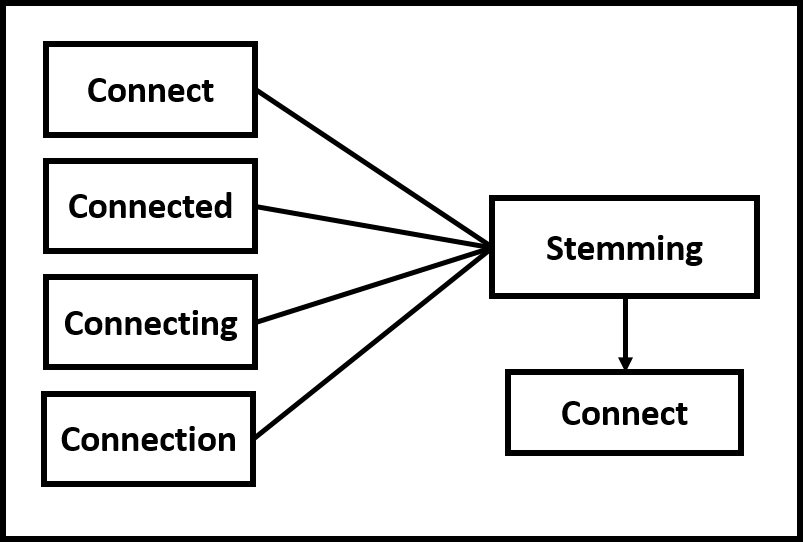
\includegraphics[width=0.45\linewidth]{01.Chapters/02.Background/stemming}
			\caption{Stemming process for ``connect'' variations, Figure from  \cite{vijayarani2015preprocessing}.}
			\label{fig:stemming}
		\end{figure}
		
		% stemming algorithms
		
		\item Lemmatization: similar to stemming, this step also reduces words to some primitive form, but with a little improvement. Lemmatization can return the words to his dictionary form, based on its part of speech context. Hence, it is possible to discriminate words with the same spelling but different meanings depending on the context. 	
				
		\item Remove stop words:
		Many words can occur a several time in a document without adding any meaningful information, such as \textit{the}, \textit{is}, \textit{at}, \textit{which}, and \textit{on}. Their high frequency can be identified as an obstacle to perform good results on NLP models, \cite{kannan2014preprocessing}. 
		
		There are some types to remove stop words, most of then based on evaluating the frequency of words in a text, for more information see \cite{vijayarani2015preprocessing}. But the classic and easier method is based on using a pre-compiled list of know words and removing then from the text.
		
		\item Everything else:
		Different from the previous steps, the last one doesn't need any grammar rules or even a frequency analysis, it's purely text manipulation. It involves set all character to lowercase; remove numbers or convert then to word form; remove punctuation; expand contractions; convert special characters to ASCII form; and any other conversion needed.		 	
	\end{enumerate}
	
	\subsubsection{Tokenization}
	Once the data is normalized, we need to know how to represent it. The tokenization process consists in splitting longer strings into meaningful small pieces called tokens. The most common way to tokenize a text is chunking it the into words, i.e., given a piece of text the tokenization process will return a list of words. 
	
	\subsubsection{Bag of Words}
	The machine learning algorithms take numerical features as input, hence, it will be necessary to represent the text in numerical form. With the Bag of Words model, we can represent in matrix form a set of documents.
	
	With the tokenization output, we will have the lists representations for all documents in the data set. Those lists can be interpreted as vectors over the vector space of all unique tokens, also called by vocabulary. So, for a given sentence, we mark how many times its words appear in the list indexes where each entry corresponds to a word in the vocabulary. Figure \ref{fig:bag-of-words} shows a simple example of how three sentences can be represented with the BoW model.
	
	\begin{figure}[h!]
		\centering
		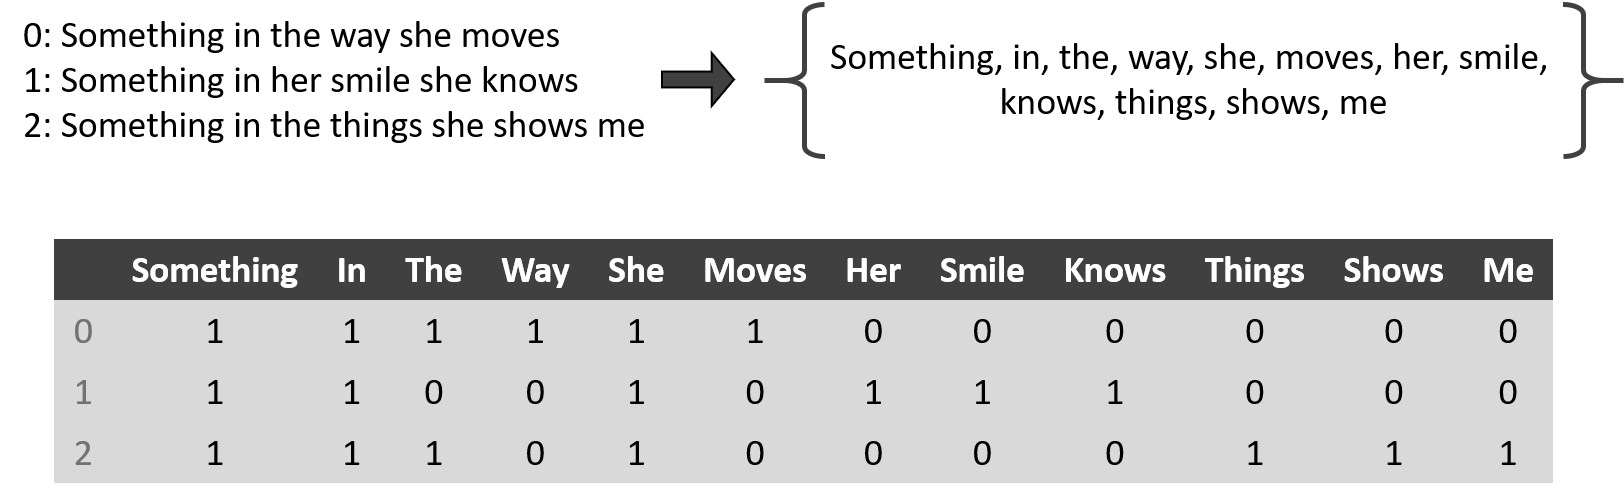
\includegraphics[width=\linewidth]{01.Chapters/02.Background/bag-of-words}
		\caption{Bag of Words example.}
		\label{fig:bag-of-words}
	\end{figure}
	
	\subsubsection{TF-IDF}
	
	Term Frequency Inverse Document Frequency, TF-IDF for short, it is applied to a BoW to determine the relative frequency for words in a specific document when compared to the inverse proportion of that word over all documents in the collection. So, it can be determined how important are the words in a specific document. 
	
	From BoW, for the $i^{\text{th}}$ vocabulary's word in the $j^{\text{th}}$ document, its TF-IDF weight is:
	
	\begin{equation}
	\label{eq:tf-idf}
	w_{i, j} = \text{tf}_{i, j} \times \log\left(\dfrac{N}{\text{df}_{i}}\right) \text{.}
	\end{equation}
	
	Where, the term frequency, $\text{tf}_{i, j}$, is how many time $i^{\text{th}}$ word appears in the $j^{\text{th}}$ document. The document frequency, $\text{df}_{i}$, is the number of documents in which th $i_{\text{th}}$ vocabulary words is present. And, finally, $N$ is the size of the document collection, with a large number of documents this term can explode, so the logarithmic function is applied to dampen this effect.
	
	\subsection{Word Embedding}
	
	The vectorization methods like BoW and TF-IDF can be very useful, but they can not represent the context of the words. This means the same words used in different contexts have the same representation, just as different words used with the same meaning are represented differently. Besides that, an one-hot encoding method, like BoW, presents a very sparse representation with high dimensionality. 
	
	Word Embedding is a technique to represent words in vectors capable of capture the words context in a document. It is also capable to smooth the high dimensionality effect by using a much more compact vector to represent the words. 
	%We can use word embedding techniques as a text processing step before performing a classification, to archive better results.
		
	There are three most known ways to perform a good word embedding. We will describe briefly each one of them below. 
	
	\subsubsection{Word Representations in Vector Space}
	
	The first great word embedding technique emerged when Google researchers proposed two architectures to build continuous vector representations of words. Word's context can be observed as the words that surround it in a sentence. Then, using shallow neural networks, it is possible to calculate the word vector space based on the word's context, \cite{mikolov2013efficient}.
	
	\begin{figure}[h!]
		\centering
		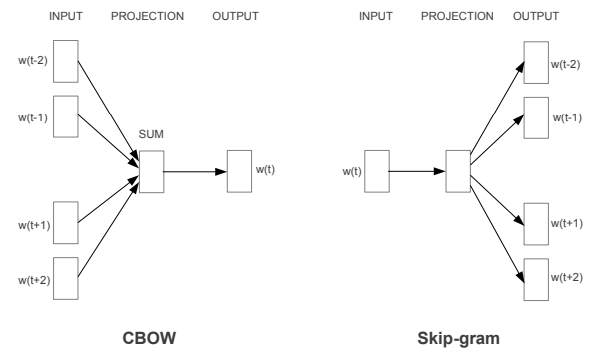
\includegraphics[width=0.7\linewidth]{01.Chapters/02.Background/word2vec_architectures}
		\caption{Word2Vec architectures, Figure from  \cite{mikolov2013efficient}.}
		\label{fig:word2vecarchitectures}
	\end{figure}
	
	The first suggested approach is the continuous bag of words or CBOW, the left side of Figure \ref{fig:word2vecarchitectures} shows its architecture. Here the neural networks are designed to predict, given the context, which word is most likely to appear. So, words with the same probability to appear can assume a shared dimension in the words vector space. 

	The second approach is known by Skip-Gram, architecture at right in Figure \ref{fig:word2vecarchitectures}. Very similar to CBOW, but instead of predicting the current word the Skip-Gram uses the current word as an input to a neural network to predict its context.
	
	% INCREMENTO: Explicar processo de treinamento, input/output e hidden layers
	
	After the network training process, we can use the hidden layer weight matrix as a lookup table to build the word embedding representation. The dimension for the vector space is managed by the number of neurons in the hidden layer. 		
	
	% INCREMENTO: Detalhes do artigo - base utilizada e testes
	
	\subsubsection{Global Vectors for Word Representation} % 
	
	Just a year later \citeonline{pennington-etal-2014-glove} arrives with a new approach to represent words in a vector space. The Global Vectors for Word Representation, or GloVe, method emerged by the need to consider some factors ignored by Skip-Gram.
		
	Methods such as Skip-Gram learn their embedding by targeting words to their respective context, ignoring the fact that some words appear more in a context than others. Thus, this co-occurrence of words only adds more useless training examples, increasing the training complexity without adding relevant information.
	
	GloVe, however, proposes to use the corpus statistics more efficiently. Using a weighted least squares model trained on a global word-word co-occurrence counts matrix. Thereby, it is possible to build a lookup table for the words in vocabulary and use it to represent them in a vector space.
	
	% INCREMENTO: Explicar processo de montagem das co-ocorrencias e probabilidades
	
	\subsubsection{Word Vectors with Subword Information}
		
	Both Skip-Gram and GloVe provide a good vector representation for words, but there still is an unsolved problem, What to do with unknown words? To solve this question was proposed a new embedding technique which uses subword units to build a vector space, \cite{bojanowski2017enriching}.
	
	Similar to Skip-Gram, this new method, the FastText, train its embedding by using a target to predict the context. However, instead of using the full words FastText goes a level deeper, breaking the words in $n$-grams, i.e., the word becomes its own context. The Figure \ref{fig:apple-tri-gram} shows how the word ``apple'' can be broken into $n$-grams. 
		
	\begin{figure}[h!]
		\centering
		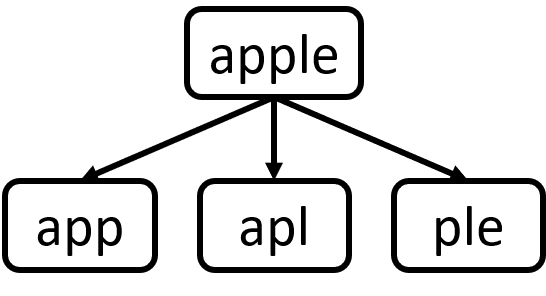
\includegraphics[width=0.3\linewidth]{01.Chapters/02.Background/apple-tri-gram}
		\caption{Tri-gram representation for ``apple'' word.}
		\label{fig:apple-tri-gram}
	\end{figure}
	
	There are a couple great advantages by using this method. It is now possible to generalize new words, or unseen in training data, since they have the same characters as known ones. Although it is possible to use available pre-trained models, the FastText requires less text to be trained, it can extract much more information from small pieces of text.	
	
	\subsection{Topic Modeling}
	
	In text-mining, we often have document collections that we want to split into similar groups or even classify them related to each other. In this way, topic modeling is an unsupervised classification tool frequently used in text-mining to identifying the hidden patterns, called ``topics'', in this document collection which carries consistent semantic meaning.
	
	Clustering methods, like hierarchical clustering, can be used to group the document collection into similar clusters. However, with a large amount of data a simple document clustering is not enough, because the semantic level of topics is not taken into account. To accomplish the topic modeling task a more sophisticated method is required, so methods like Latent Dirichlet allocation.
	
	Latent Dirichlet allocation, or LDA for short, is a probabilistic model that uses a Dirichlet distribution to model both the topics and the words. In LDA, each item in the collection is modeled as a mixture over an underlying set of topics. And the topics, in this way, is modeled as a mixture of words over the vocabulary, \cite{blei2003latent}.
		
	Without going too deep into the math behind the model, we can easily understand the two most basic principles that guide LDA. The first one said the documents are a mixture of topics which means that in a topic space each document could be interpreted as a linear combination of these topics, however, each one of the documents must be the most homogeneous as possible. The second principle said the topics are formed as a combination of words, i.e., documents about the same topics must share similar words, and also words distribution must be the most homogeneous as possible.
	
	\begin{figure}[h!]
		\centering
		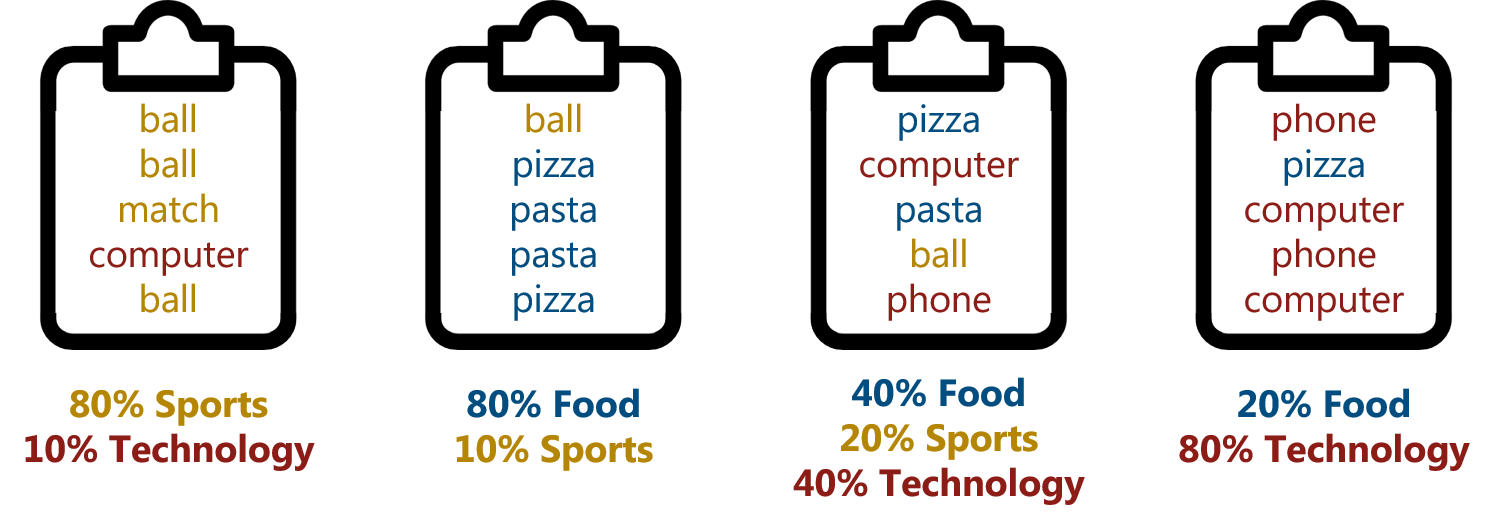
\includegraphics[width=0.85\linewidth]{01.Chapters/02.Background/topic_modeling}
		\caption{Document collection modeled by topics.}
		\label{fig:topicmodeling}
	\end{figure}
	
	Take the Figure \ref{fig:topicmodeling} as an example. It shows a little fictitious document set compounded for six words ``ball'' and ``match'' which can represent the Sports topic, ``pizza'' and ``pasta'' for the Food topic end, finally ``computer'' and ``phone'' for the Technology  topic. In this case, each word belongs to one topic, but that is not a rule, each topic is formed by a mix of words, and the documents a combination of topics.
		
	A final remark for the topic modeling algorithms is that the topic is not discovered by names, the machine only discovers the distribution of the words by topics but not which one is. It's human work to label the topic once they are found.
	
	\subsubsection{Generative Process}
	
	To better understand this model, we will analyze the generative process for creating the document collection illustrated by Figure \ref{fig:lda-generative-process}. Let's assume we have specified who the available topics are and their respective word distributions (far left), besides the topic proportions for each of the documents in the collection (the histogram at right). 
		
	\begin{figure}[h!]
		\centering
		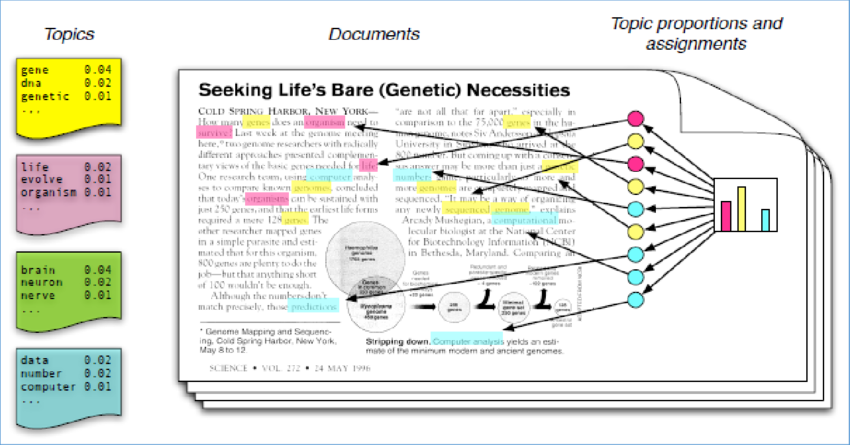
\includegraphics[width=\linewidth]{01.Chapters/02.Background/The-intuition-behind-LDA-Generative-process-by-D-Blei-17}
		\caption{The intuition behind LDA Generative process, Figure from  \cite{blei2012probabilistic}.}
		\label{fig:lda-generative-process}
	\end{figure}
	
	To generate a single document we choose its words as follows. Randomly choose a topic assignment from the topic distribution, then we choose the word from the corresponding topic. As shown by Figure \ref{fig:generative-probs} we can describe the generative process for a given $\alpha$ and $\beta$ parameters.
	
	\begin{figure}[h!]
		\centering
%		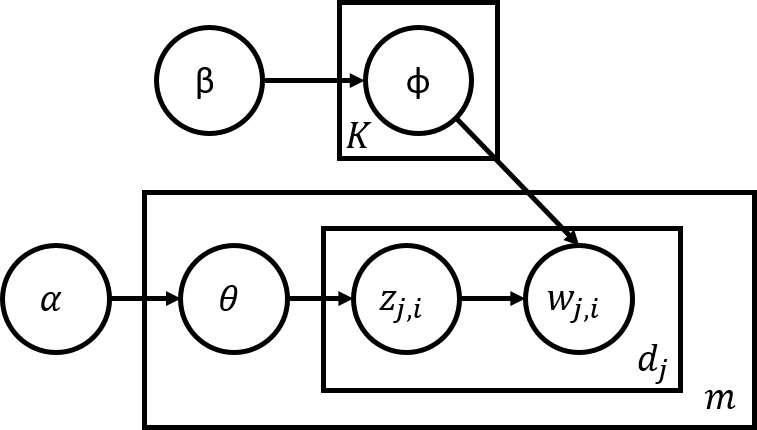
\includegraphics[width=0.5\linewidth]{01.Chapters/02.Background/generative-probs-stack}
		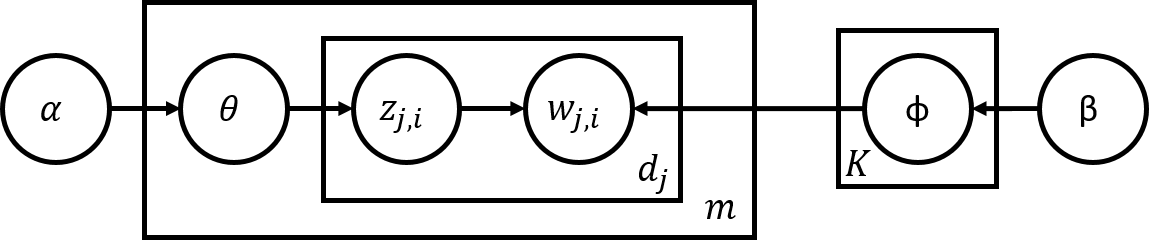
\includegraphics[width=0.7\linewidth]{01.Chapters/02.Background/generative-probs}
		\caption{Mathematical representation for LDA Generative process.}
		\label{fig:generative-probs}
	\end{figure}
	
	With that, we can model the generative process by: 
	
	\begin{equation}
		\label{eq:generative-lda}
		p(w|\alpha, \beta) = \prod_{k=1}^{K} p(\phi_{k}|\beta) \prod_{j=1}^{M} p(\theta_{j}|\alpha) \left( \prod_{i=1}^{V}p(z_{j,i}|\theta_{j}) p(w_{i,j}|z_{i,j},\phi_{z_{j,i}})  \right) \text{.}
	\end{equation}

	Where $\phi$ is the distribution of $V$ words over the $K$ topics and $\theta$ is the topic distribution over the $M$ documents. The term inside the parentheses represent the choice of a word $w$ for a document given the assignment of topics $z$ for the specific document.
	
	\subsubsection{Model Inference}
	
	The inference process for LDA consists of finding the best fit of the distribution $\phi$, for words over topics, the distribution $theta$, for topics over documents, and the assignment $z$ for each document in the collection given the words vectors representation, usually a bag of words model, and the hyperparameters $\alpha$ and $\beta$, who are the Dirichlet parameters for respective $\theta$ and $\phi$ distributions.
	
	Given the expensive computational cost, we can use some techniques to infer the LDA, the most common one is the Gibbs Sampling. This method is an algorithm for obtaining a sequence of observation which are approximated from a specified multivariate probability distribution. In easy words, showed by \citeonline{faleiros2016modelos}, the Gibbs sampler will iterate over the documents and its words to compute the relations:

	\begin{equation}
		\label{eq:theta-dist}
		\theta_{k} = \frac{C_{w,k}^{NWZ} + \beta_{w}} {\sum_{w_{-i}} \left(C_{w_{-i},k}^{NWZ} + \beta_{w^{'}} \right)} \text{,}
	\end{equation}
	
	\begin{equation}
		\label{eq:phi-dist}
		\phi_{d} = \frac{C_{d,k}^{NZM} + \alpha_{k}} {\sum_{k'}^{K} \left(C_{d,k^{'}}^{NZM} + \alpha_{k^{'}} \right)} \text{.}
	\end{equation}

	Where $C_{w,k}^{NWZ}$ is the counter of times a word $w$ is assigned to topic $k$; and $C_{d,k}^{NZM}$ is the counter of times a topic $k$ is assigned to a word in a document $d$. The Algorithm \ref{algo:gibbs-sampling} shows in a simple way how the Gibbs sampling works to infer the LDA distributions.
	
	\begin{algorithm}[h!]
		\caption{Gibbs sampler} 
		\label{algo:gibbs-sampling}
		\begin{algorithmic}[1]
			\State \textbf{input:} number of topics $K$, document collection, $\alpha$ and $\beta$
			\Begin
			\State Initialize the counters randomly;
			\While{Did not converge}
			\For{document $m \in [1, D]$}
			\For{word $n \in [1, N_{m}]$ in document $m$}
			\State $nwz[w_{m,n}, z_{m,n}]--$; $nz[z_{m,n}]--$; $nzm[z_{m,n},m]--$;
			\State Sample a topic $z_{m,n}$ according to the previous equation
			\State $nwz[w_{m,n}, z_{m,n}]++$; $nz[z_{m,n}]++$; $nzm[z_{m,n},m]++$;
			\EndFor
			\EndFor
			\If{converged $L$ since the last sampling}
			\State calculate the distributions $\theta_{k}$ and $\phi_{d}$;
			\EndIf
			\EndWhile
			\End
		\end{algorithmic} 
	\end{algorithm}
	
	\subsubsection{Evaluating Topic Models}
	
	After approximating LDA's distribution, we will have $K$ topics represented like distributions over the vocabulary. To interpret the found topics, we use the most likely words to co-occur, usually the top 10 or 15 with high probability. However, the $K$ parameter is a model input, so the wrong choice for it could result in unmeaningful topics. 
	
	To evaluate properly the good interpretability for a topic model, there are some topic coherence metrics. The concept behind topic coherence consists of measuring the degree of semantic similarity between high scoring words in the topic. Then, a topic is considered to be coherent if its main words are related.
	
	There are several topic coherence metrics to evaluate interpretability for topic models, \citeonline{newman2010automatic} presents and compares some of them.
	% and \citeonline{rosner2013evaluating} studies	the $C_{\text{umass}}$ score based on document coocurrence counts. 
	Despite this, according to \citeonline{syed2017full}, the coherence metric, labeled by $C_{\text{V}}$, achieves the highest correlation with all available human topic raking data. The calculation for $C_{\text{V}}$ metric is based on four steps:
	
	\begin{enumerate}
		\item Segmentation of the data into word pairs, combining each topic's top-N words with every other top-N word;
		
		\item Calculation of word or word pair probabilities, $p(w_{i})$ or $p(w_{i}, w_{j})$, respectively. That probability is calculated as the percentage of documents in which $(w_{i})$ or $(w_{i},w_{j})$ occurs, ignoring the frequencies and distances between words;
		
		\item Calculation of a confirmation measure $\phi$ that quantifies how strongly a word set supports another one, based on the normalized pointwise mutual information $\text{NPMI}$, for each segmented pair $S_{i}$. These confirmation measures can be calculated by:
		
		\begin{equation}
			\vec v (\text{W}') = \left\{ \sum_{w_{i} \in \text{W}'} \text{NPMI} (w_{i}, w_{j})^{\gamma} \right\}_{j=1,...,|\text{W}|} \text{,}
		\end{equation}
	
		\begin{equation}
			\text{NPMI} (w_{i}, w_{j})^{\gamma} = \left( \dfrac{\log \frac{P(w_{i}, w_{j}) + \epsilon}{P(w_{i}) \cdot P(w_{j})} }{- \log (P(w_{i}, w_{j}) + \epsilon) } \right)^{\gamma} \text{,}
		\end{equation}
	
		\begin{equation}
			\phi_{S_{i}}(\vec u , \vec w) = \dfrac{ \sum_{i=1}^{|\text{W}|} u_{i} \cdot w_{i} }{||\vec{u}||_{2} \cdot ||\vec{w}||_{2}} \text{.}
		\end{equation}
	
		Where $\epsilon$ and $\gamma$ are parameters to, respectively, account the zero logarithm and place more weight on higher $\text{NPMI}$ values. The vector $\vec{v}(\text{W}')$ is called by context vectors.
	
		\item Finally, aggregation of individual confirmation measures into an overall coherence score, i.e., apply the arithmetic mean for all confirmation measures.
	\end{enumerate}
	
\section{Machine Learning}
	
	The basics behavior for a Machine Learning (ML) algorithm consists of building mathematical models based on data, usually known by training data, to provide predictions without being explicitly programmed to this, i.e., just knowing the training data, the model learns to make new predictions. 
	
	When the entries for our training data have a label, used to guide the learning algorithm, we are facing a supervised learning method. Digging a little deeper, our problem could consist in classification when the labels are restricted to a limited set of values; or regression when the labels could have any numerical value in range. 
		
	\subsection{Classification}
	
	As a usual ML problem, a classification task consists of building a model to fit some training data set. In a classification model, we make predictions for the class of given data points, when we have only two classes, let's call then by the positive and negative, we are facing a binary classification problem.
	
	There are several algorithms that we can use to build a classifier from the simple k-nearest neighbor until the more sophisticated ones like decision trees, naive bayes, support vectors machines, and artificial neural networks. Although each of these methods has its particularities in their formulation, they are capable of fitting the training data to make new predictions based on them.
	
%	\subsubsection{Naive Bayes}
	
%	\subsubsection{Support Vector Machine}
		
	\subsection{Evaluating a classifier}
	
	After the training step, we need to evaluate our classifier to verify how good our model is fitting the training data. The easiest way to evaluate our model is by reserving a split of the training set, the holdout set, exemplified in Figure \ref{fig:holdout-evaluate}. So, we use this unseen data to test the model and compute a metric.
	
	\begin{figure}[h!]
		\centering
		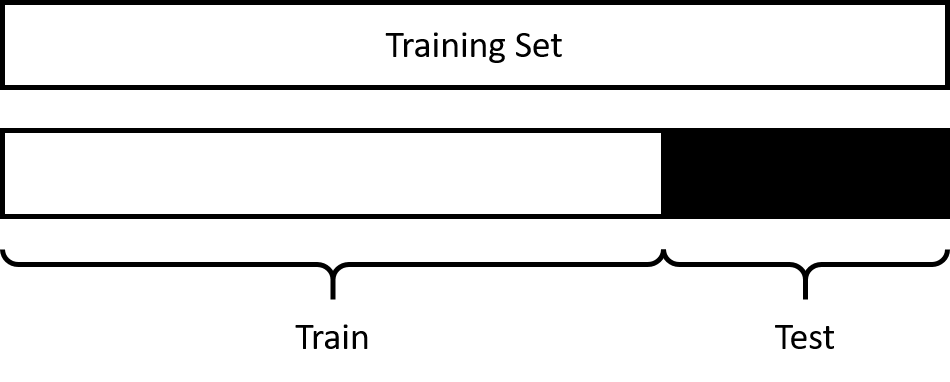
\includegraphics[width=0.4\linewidth]{01.Chapters/02.Background/holdout-evaluate}
		\caption{Train test split for holdout method.}
		\label{fig:holdout-evaluate}
	\end{figure}

	Another way to evaluate the model is through the $k$-fold cross-validation method, shown in Figure \ref{fig:cross-validate}. Dividing the data set into $k$ folds with the same size, we can train the model with $k-1$ folds and use the remaining one to test. Then we repeat this process to each fold and average the metric to evaluate the model.

	\begin{figure}[h!]
		\centering
		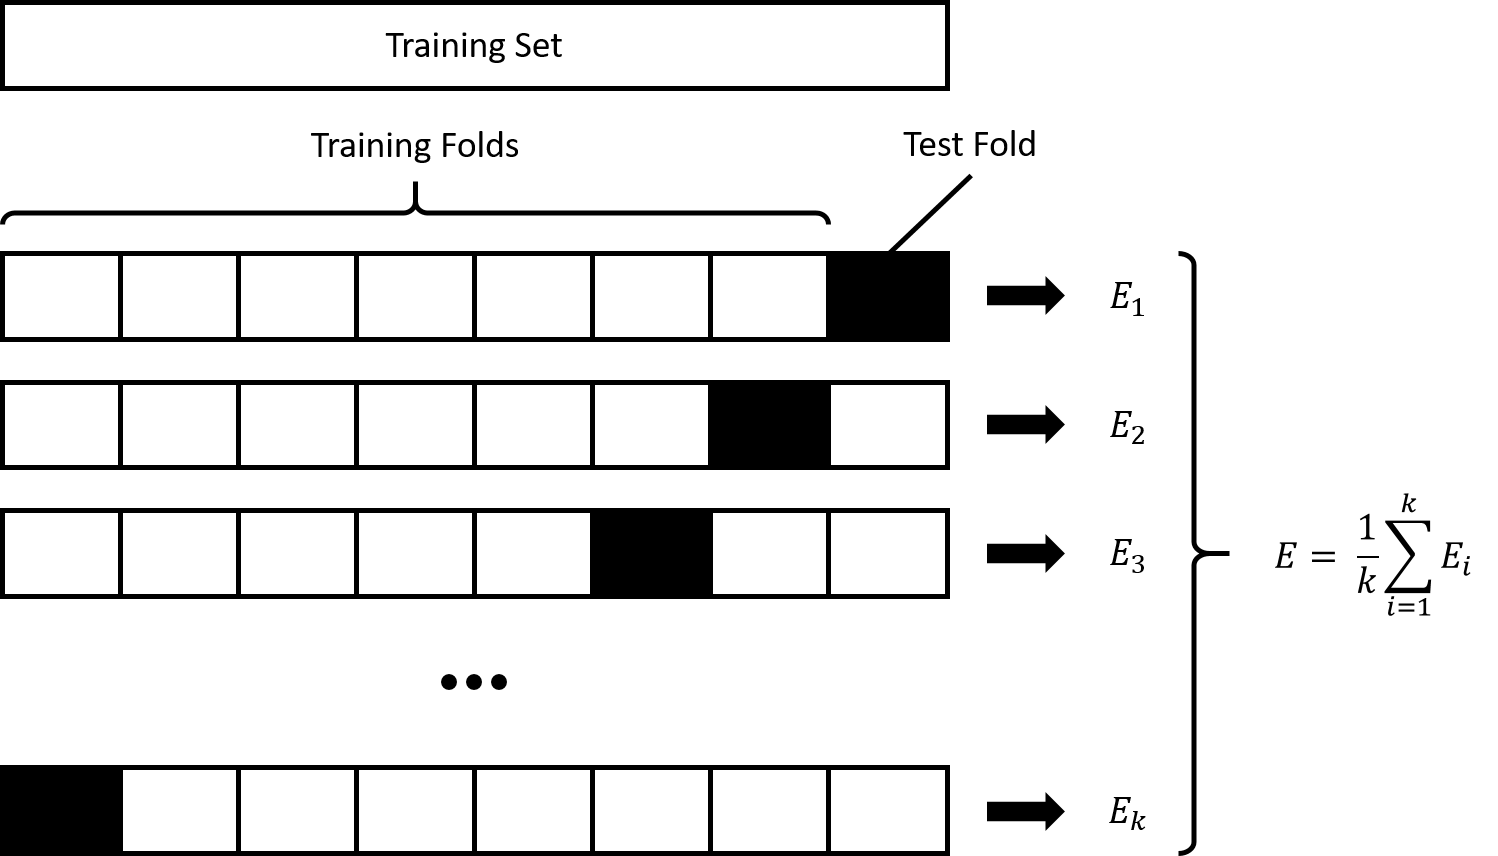
\includegraphics[width=0.55\linewidth]{01.Chapters/02.Background/cross-validate}
		\caption{Cross-validation process.}
		\label{fig:cross-validate}
	\end{figure}
	
	\subsubsection{Metrics}
	\label{sub-sub:metrics}

	Given the evaluation techniques, we still need a metric to properly evaluate the model. To present the main metrics, let's first take a brief look at the confusion matrix. Table \ref{tab:conf-matrix} exemplifies the confusion matrix for binary classification, each row represents the entries in a predicted class and the columns represent the actual class for the entry points.
	
	\begin{table}[h!]
		\centering
		\caption{Binary classification confusion matrix.}
		\label{tab:conf-matrix}		
		\begin{tabular}{cc|c|c|}
			\cline{3-4}
			&          & \multicolumn{2}{c|}{Actual Class} \\ \cline{3-4} 
			&          & Positive        & Negative        \\ \hline
			\multicolumn{1}{|c|}{Predicted} & Positive & TP              & FP              \\ \cline{2-4} 
			\multicolumn{1}{|c|}{Class}     & Negative & FN              & TN              \\ \hline
		\end{tabular}
	\end{table}

	Thus, we can have the true positives (TP) and true negatives (TN) when our model makes a good prediction about the positive and negative classes, respectively, when the model misses the prediction we call false positive (FP) or false negative (FN). 
	
	\begin{enumerate}
		\item \textbf{Accuracy:} The simplest metric, extracted from the confusion matrix, shows us the percentage of correct predictions by the relation:
		
		\begin{equation}
			Accuracy = \frac{TP + TN}{TP + FP + TN + FN} \text{.}
		\end{equation}
		
		\item \textbf{Precision:} In some cases, like a very imbalanced scenario, the accuracy is not good because even if the model predicts all the instances by the predominating class we will still have high accuracy. We define the precision of the positive class by:
		
		\begin{equation}
			Precision(P) = \frac{TP}{TP + FP} \text{.}
		\end{equation}
	
		Thus, we will analyze the true predictions only by the positive predicted class.
		
		\item \textbf{Recall:} This metric represents the fraction from a class that is correctly predicted. We define the recall for the positive class by:
		
		\begin{equation}
			Recall(P) = \frac{TP}{TP + FN} \text{.}
		\end{equation}
		
		Similar to precision the recall for the positive class will compare the true predictions by the total count of true actual classes.
		
		\item \textbf{F1 Score:} In some cases, we may want to give the same importance to both precision and recall. A popular metric to combine then is called F1-score, which is the harmonic mean of precision and recall. We define the F1-score for the positive class by:
		
		\begin{equation}
			F1(P) = \frac{2 \times Precision(P) \times Recall(P)}{Precision(P) + Recall(P)} \text{.}
		\end{equation}
	
	\end{enumerate}
	
	

\chapter{Related Works}\label{chap:related}
In the last chapter, we saw the theoretical foundation of NLP techniques. In this chapter, we will review in the literature some works that employ the NLP techniques described to discover topics in a data set. In addition, we will show some applications for this type of task. And, finally, some final remarks to continue this work.


\section{Topics Discovery}

Finding meaningful topics in a document collection has been used for many authors for the most various applications. For example, \citeonline{hurtado2016topic} use topic modeling to inspect research publications, patents, and technical reports aiming to model the evolution of the direction of research and forecast the near future trends in IT industry.

Using the titles and abstracts of a data set with more than six thousand academic papers between 2002 and 2010, mostly collected by \citeonline{tang2008arnetminer}, they proposed a sentence-level association rule to discover meaningful topics. After categorizing the documents in topics, they were capable of building time series for each found topic, marking how many times that topic was cited in a given year. So, they were able to build an ensemble of forecasters to study the patterns and relationships among topics over the years.

For a better understanding, Figure \ref{fig:topic-discovery-framework} has a flowchart with their proposed framework for the topic discovery and forecasting.

\begin{figure}[h!]
	\centering
	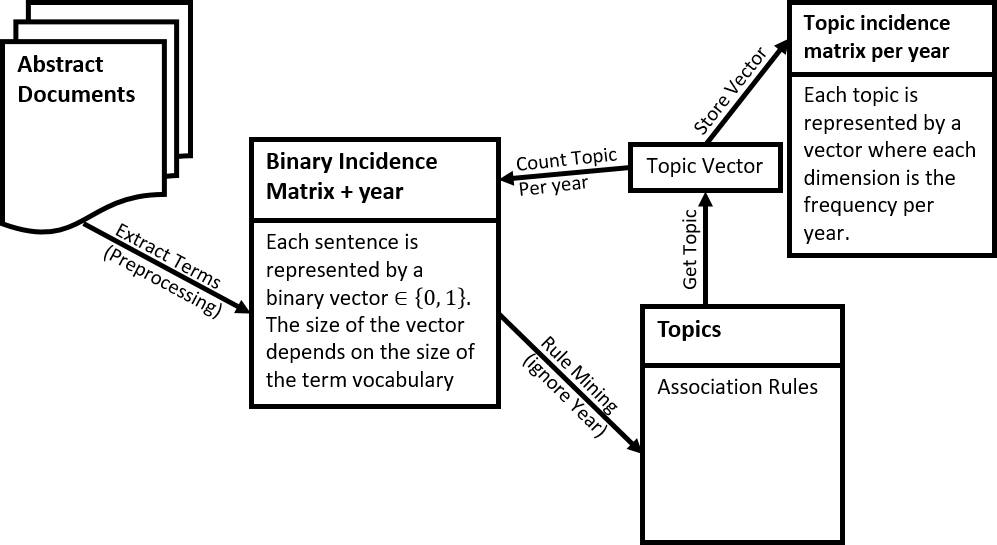
\includegraphics[width=0.6\linewidth]{01.Chapters/03.RelatedWorks/topic-discovery-framework}
	\caption{Flowchart of the proposed framework, Figure from  \cite{hurtado2016topic}.}
	\label{fig:topic-discovery-framework}
\end{figure}

This framework involves some well-known major steps of NLP processing. First, they convert the documents into a transactional form, i.e., the phrases in each document will be considered individually during the process. Next, they perform the basic normalization steps which include case conversion, tokenization, removing step words, part of speech tagging, stemming and lemmatization. It is also performed an additional step, specific to their application, removing verbs such as ``exploiting'', ``adapting'' and ``propose'', because they are very common in scientific publications and do not add much meaningful information.

To vectorize the transactions, it is used a slight variation of BoW. Instead of word counting, it is only checked whether a word belongs to a transaction, this is called the binary incidence matrix. The topic discovery step comes afterward, applying an association rule mining to the transactions and discovery their patterns. In order to avoid different topics with redundant words is applied a rule refinement process that allows similar topics to be combined.

Online forums and social media are excellent platforms for people to discuss and share information about a variety of subjects. Recently, the topic discovery technique was used to summarize different topics related to COVID-19 disease and perform a sentiment analysis on them~\cite{jelodar2020deep}.

Reddit is a discussion website in which its users can submit posts and start discussions with other community members. The posts are organized in the called ``subreddits'', boards created by users to discuss a specific subject. Using over half a million comments from 10 health-related subreddits with information about COVID-19, \citeonline{jelodar2020deep} performed a topic discovery to group similar comments. So, applying a sentiment analysis on each comment it was possible to summarize the average opinion about the discovered topics.


\section{Trend Forecast}

Predicting future trends can be very helpful in various applications, like to model the evolution of research. Following the topic discovery process from \citeonline{hurtado2016topic}, a forecast trend was used to predict the near future related to each discovered topic. With all documents belonging to at least one identified topic in the set, was created a topic incidence matrix that contains the count of times a topic is mentioned over the years. Finally, they make an ensemble forecasting to predict the future topic counting using the framework shown in Figure \ref{fig:ensemble-forecasting-framework}.

\begin{figure}[h!]
	\centering
	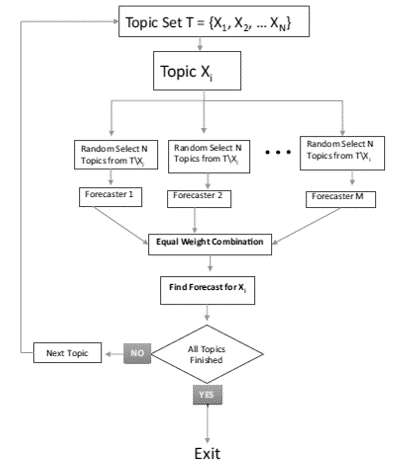
\includegraphics[width=0.5\linewidth]{01.Chapters/03.RelatedWorks/ensemble-forecasting-framework}
	\caption{Ensemble forecaster framework, Figure from  \cite{hurtado2016topic}.}
	\label{fig:ensemble-forecasting-framework}
\end{figure}

Given a specific topic, they generate $M$ forecasters which target $X_{i}$ along with N randomly chosen fields, excluding $X_{i}$. Then, the predicted value, $\hat{X}_{i}(t+1)$, is an average of each individual forecast, $\hat{X}_{i, F_{k}}(t+1)$, calculated by 

\begin{equation}
	\hat{X}_{i}(t+1) = \dfrac{1}{M} \sum_{k=1}^{M}\hat{X}_{i, F_{k}}(t+1)\text{.}
\end{equation}

By evaluating metrics like the coefficient of determination (R-squared) and mean squared error (MSE) they were able to conclude the ideal number $N$ of variables to predict more accurately the future for all topics in the set.

\citeonline{shentopic} also predicted trends by analyzing the exponential growth in the volume of scholarly articles published over the years. However, he skips the NLP process step by using a pre-labeled data set from Springer containing the number of works above 14 subjects in 25 years. Using an ensemble forecast based on neural networks and support vector regression he was able to study the topics' growth and codependency between them.


\newpage
\section{Final Remarks}

As we saw earlier topic discovery and trend forecast were subjects widely explored in the literature. With that in mind, we wish, in this work, to reproduce these techniques. However, in addition to what has been presented, we want to be able to explore some modifications.

Assuming a system that receives documents in real-time, let's assume they are news, it would be very computationally expensive to redo all the topic discovery process with each new news. It would be much simpler if there was a process that, given an input document, would be able to identify 
which topics were covered by it.

So, aiming at this type of application, we will propose a system capable of such activity to model the topics evolution over time.




%\chapter{Materials and Methods from tg-1}\label{chap:materials-1}
%In this chapter, we will discuss the roadmap steps to carry out this work. First, we will reintroduce the work objectives. Finally, the work plan with the necessary steps to accomplish the proposed objectives.

\section{Objective}

As already discussed, we want to build models capable of making predictions regarding the evolution of discovered topics in a set of documents. We also want to find topics in real-time at each received document without having to redo the topic discovery process. Then, by the end of this work, we must have performed the tasks listed below.

\begin{itemize}
	\item Find a database long enough, over several years;
	\item Perform all necessary treatment steps to normalize the documents' texts;
	\item Find meaningful topics in a subset from the original database;
	\item Create a topic classifier to find out if a document addresses any topic of interest;
	\item Model topic evolution to evaluate the forecast accuracy.
\end{itemize}

\section{Research method}

With the objectives defined, we must have action plans to achieve them. Next, we will discuss in more detail the action plan for each of these previous punctuated steps.

We need to mention the figure notation used in the next sections. Whenever a box with the bottom right tip folded appears, it represents a machine learning process with all the applicable steps, such as cross-validation and hyperparameter tuning.

\subsection{Database}

The first necessary task is to find a database over several years. Some options are available, such as daily news from Wikipedia, newspaper articles, research and academic papers, patents, and even social media data like Twitter or Reddit. We must be careful to choose a database that covers several years in order to get a good temporal representation when modeling their topics.

\subsection{Pre-processing the data}

With the chosen database, we must define a data pre-processing pipeline to normalize the documents, putting all of then at the same pattern. For this, we can use the normalization techniques shown in Chapter \ref{chap:literature} like stemming, lemmatization, stop words removal, and all necessary textual manipulations to obtain the best text representation for the documents.

After processing the data, we need to index then over the time and, then, split the full treated data set in three subsets. They must be time ordered, as shown in Figure \ref{fig:database}, this means that for each document in $T_{i}$ its time index $t_{x}^{(i)}$ must be lower then any index $t_{x}^{(m)}$ in a document contained in $T_{m}$, and so on.

\begin{figure}[h!]
	\centering
	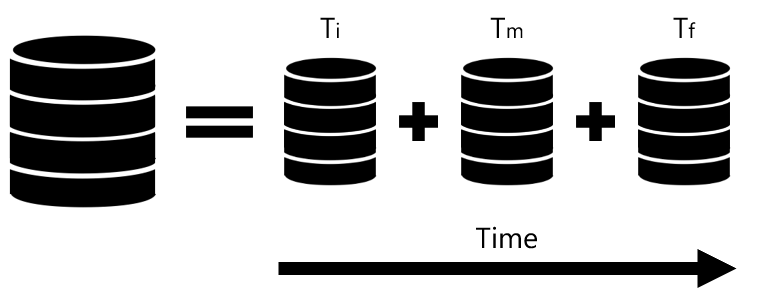
\includegraphics[width=0.6\linewidth]{01.Chapters/04.Materials/database}
	\caption{Database time split representation.}
	\label{fig:database}
\end{figure}

Before proceeding, let's name the subsets. The initial subset will be called \textit{Identifier} from now on, the middle and final ones will be respectively designated by \textit{Modeler} and \textit{Validation}. 

\subsection{Topic identification}

With the \textit{Identifier} set, techniques of document clustering will be applied to identify the discussed subjects in the documents, the Figure \ref{fig:topic-identification} illustrates the sequence of steps for this task. Similar to \citeonline{hurtado2016topic}, a refinement will be made so that only significant topics remain. 

\begin{figure}[h!]
	\centering
	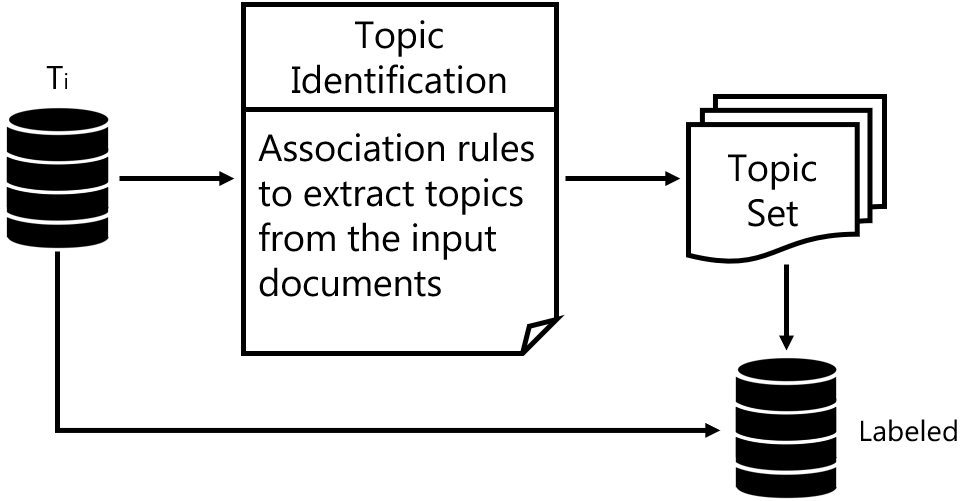
\includegraphics[width=0.8\linewidth]{01.Chapters/04.Materials/topic-identification}
	\caption{Topic identification process.}
	\label{fig:topic-identification}
\end{figure}

Next to the topic identification we will obtain a topic set, then each document contained in \textit{Identifier} can be labeled with at least one topic from the set, this new database will be called by labeled \textit{Identifier}.

\subsection{Document classification}

For each topic in our set of discovered topics, we must be able to identify which topics are covered by a new document. Thus, we will build a classifier to perform this verification.

Knowing that a document can talk about several topics, so we must have a multi-class classifier. We can see this as an individual binary classifier for each topic that tells us whether the document has it. Using the labeled \textit{Identifier} set it is possible to build this classifier. Figure \ref{fig:document-classification} illustrates it in detail.

\begin{figure}[h!]
	\centering
	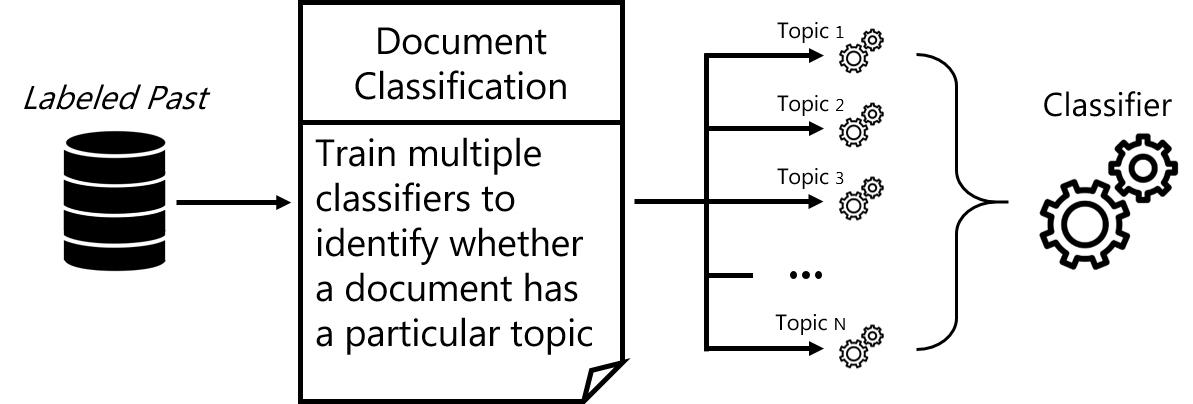
\includegraphics[width=0.9\linewidth]{01.Chapters/04.Materials/document-classification}
	\caption{Multi-class classifier from \textit{Labeled} set.}
	\label{fig:document-classification}
\end{figure}

\subsection{Forecast evaluation}

Finally, to evaluate the time series model is the last task to be accomplished. Following the flowchart shown in Figure \ref{fig:forecast}, first, we have to label the \textit{Modeler} and \textit{Validation} sets. Then, using labeled \textit{Identifier} and \textit{Modeler} we will build a topic incidence matrix over the time, to apply a forecaster process for those time series. With the labeled \textit{Validation} set we will perform an evaluation for our model and then make conclusions about it.

\begin{figure}[h!]
	\centering
	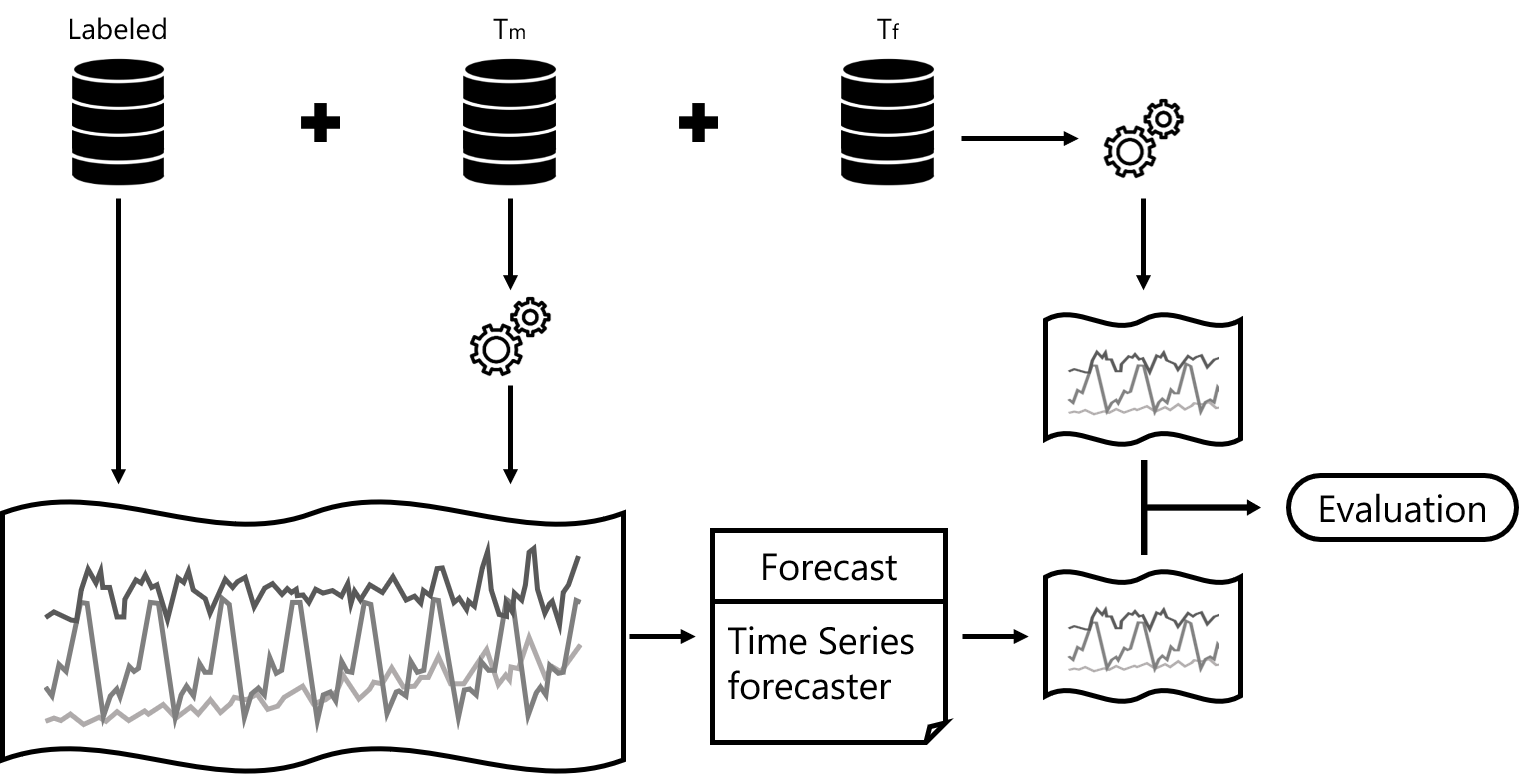
\includegraphics[width=\linewidth]{01.Chapters/04.Materials/forecast}
	\caption{Flowchart to evaluate the time series model.}
	\label{fig:forecast}
\end{figure}


\chapter{Materials and Methods}\label{chap:materials}
In the previous chapters, we presented the motivation of this work, the literature review showing the main concepts behind the work, then, we briefly described some related works. In this chapter, we will describe the problem, the whole experimentation setup, and the tools used to accomplish the proposed objectives.

\section{Database}

The first necessary task is to find a database spread over several years. For this, the Neural Information Processing Systems database was chosen, \cite{nipsweb}. With 7241 entries spread in a thirty-year range, this base contains academic papers from the NIPS conference, one of the most prestigious yearly events in the machine learning community. Table \ref{tab:dataset-description} contains the description of the main columns present in the data set.

\begin{table}[h!]
	\centering
	\caption{Main feature description for NIPS data set.}
	\label{tab:dataset-description}
	\begin{tabular}{r|lc}
		\toprule
		    Feature & Description          & Data Type \\ \midrule
		         id & Paper identifier     &  Integer  \\
		       year & Year of publication  &  Integer  \\
		      title & Title of publication &   Text    \\
		   abstract & Publication abstract &   Text    \\
		paper\_text & Publication corpus   &   Text	   \\ \bottomrule
	\end{tabular}
\end{table}

\section{Pre-processing the Data}

With the chosen database, we must define a data pre-processing pipeline to normalize the documents, putting all of them at the same pattern. For this, we can use the normalization techniques shown in Chapter \ref{chap:literature} like stemming, lemmatization, stop words removal, and all necessary textual manipulations to obtain the best text representation for the documents.

\subsection{Normalization Pipeline}

To be more specific about the normalization process, let us describe it in more detail. First of all, we must concatenate the title, the abstract, and the paper text to treat all the paper information like a single document in our corpus. Done that, we proceed with the other normalization steps in the order as follows.

\begin{enumerate}
	\item \textbf{Drop links:} drop all possible links, by regular expression, in the text that could disturb the other steps;
	\item \textbf{Remove numbers:} remove all numbers, by regular expression, in the text;
	\item \textbf{Expand contractions:} Convert some english contractions into their full form;
	\item \textbf{Remove punctuation:} Replace all punctuation marks to empty space;
	\item \textbf{Convert special characters:} Replace special characters, accented letters for example, with their ASCII form;
	\item \textbf{Case conversion:} Change all characters by their lower forms;
	\item \textbf{Lemmatization:} Convert the words to their root form by lemmatizing them according to their part of speech tag;
	\item \textbf{Remove stop-words:} Remove the english well-known stop words.
\end{enumerate}

Figure \ref{fig:normalized-text} illustrates an example of the application of the above mentioned language processing techniques to a given input.

\begin{figure}[h!]
	\centering
	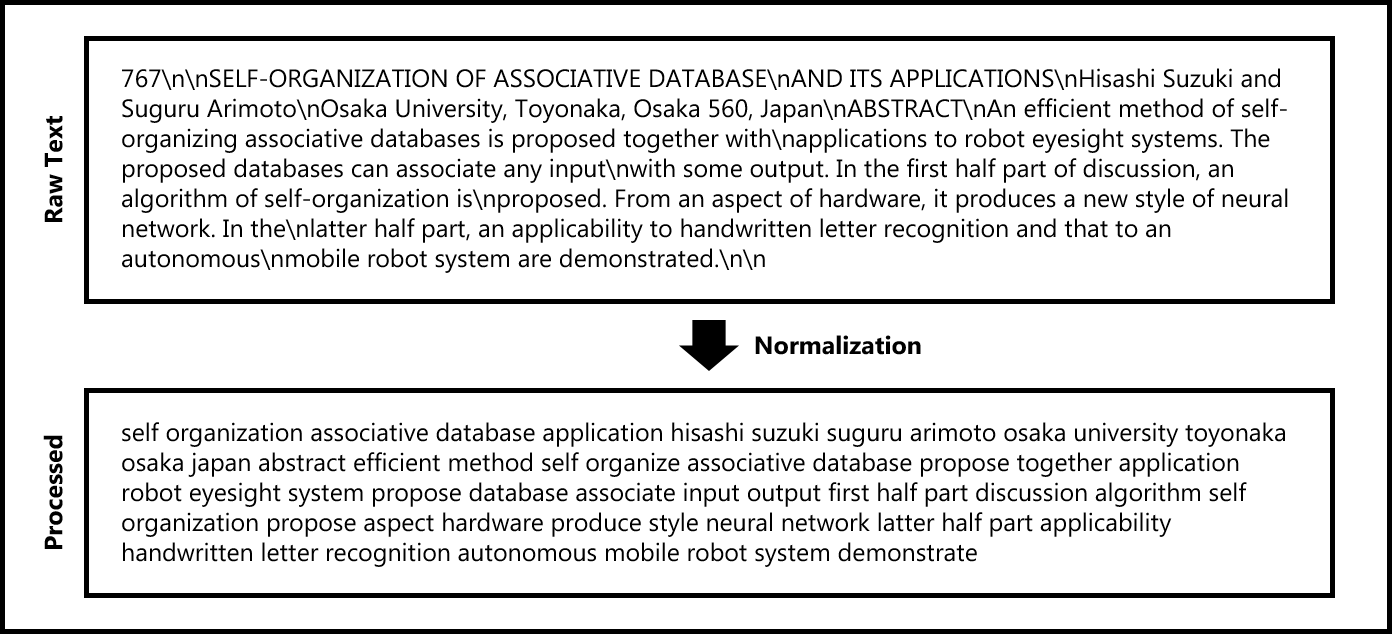
\includegraphics[width=\linewidth]{01.Chapters/04.Materials/normalization-process}
	\caption{Demonstration about the normalization process.}
	\label{fig:normalized-text}
\end{figure}

\subsection{Segmentation}

After processing the data, we need to index them over time and, then, split the full treated data set into three subsets. They must be time ordered, as shown in Figure \ref{fig:database}, this means that for each document in $T_{i}$ its time index $t_{x}^{(i)}$ must be lower then any index $t_{x}^{(m)}$ in a document contained in $T_{m}$, and so on.

\begin{figure}[h!]
	\centering
	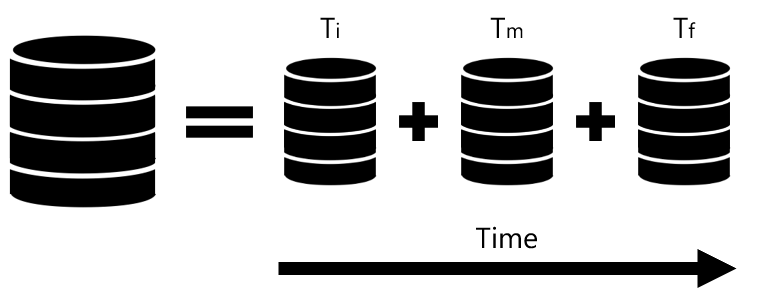
\includegraphics[width=0.7\linewidth]{01.Chapters/04.Materials/database}
	\caption{Database time split representation.}
	\label{fig:database}
\end{figure}

Before proceeding, let us give a name to the subsets. The initial subset will be called \textit{Past} from now on, the middle and final ones will be respectively designated by \textit{Present} and \textit{Future}. To segment these three subsets, let us first analyze the yearly distribution of documents. Figure \ref{fig:yearly-histogram} shows how the documents are spread over the years, and Figure \ref{fig:yearly-cumulative} shows the cumulative distribution of documents with the percentiles marks of 30\% and 80\%.

\begin{figure}[h!]
	\begin{subfigure}{0.5\textwidth}
		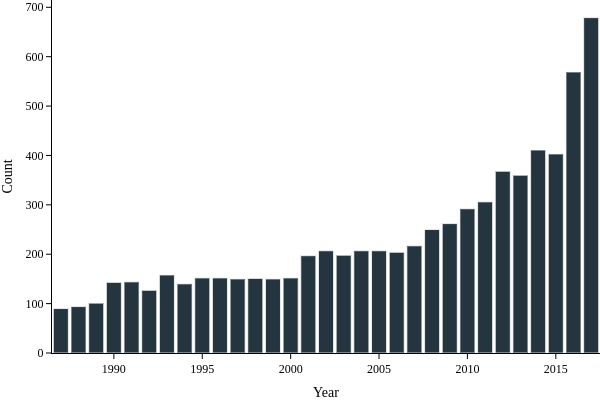
\includegraphics[width=\linewidth]{01.Chapters/04.Materials/yearly-histogram}
		\caption{Histogram for year distribution.} \label{fig:yearly-histogram}
	\end{subfigure}%
	\hfill
	\begin{subfigure}{0.5\textwidth}
		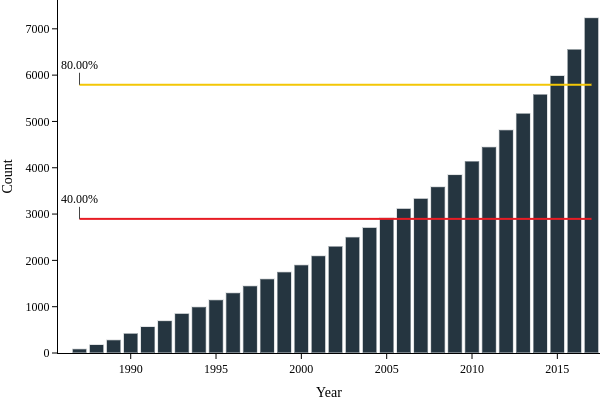
\includegraphics[width=\linewidth]{01.Chapters/04.Materials/yearly-cumulative}
		\caption{Cumulative histogram.} \label{fig:yearly-cumulative}
	\end{subfigure}%
	\caption{Yearly distribution of documents.}
	\label{fig:yearly-distribution}
\end{figure}

After this division, shown in Figure \ref{fig:yearly-distribution}, we approach the limits to 2002 and 2015. Then, the temporal division for the subsets was done as indicated in Table \ref{tab:database-description}.

\begin{table}[h!]
	\centering
	\caption{Subsets description after segmentation.}
	\label{tab:database-description}
	\begin{tabular}{r|cc}
		\toprule
		 Subset & No. of documents &    Years    \\ \midrule
		   Past &       2308       & 1987 - 2002 \\
		Present &       3685       & 2003 - 2015 \\
		 Future &       1248       & 2016 - 2017 \\ \bottomrule
	\end{tabular}
\end{table}

\section{Topic Modeling}

With the \textit{Past} set, techniques of topic modeling will be applied to identify the discussed subjects in the documents. Figure \ref{fig:topic-identification} illustrates the sequence of steps for this task. Next to the topic identification, we will obtain a topic set, then each document contained in \textit{Past} can be labeled with at least one topic from the set, this new database will be called by \textit{labeled Past}.

\begin{figure}[h!]
	\centering
	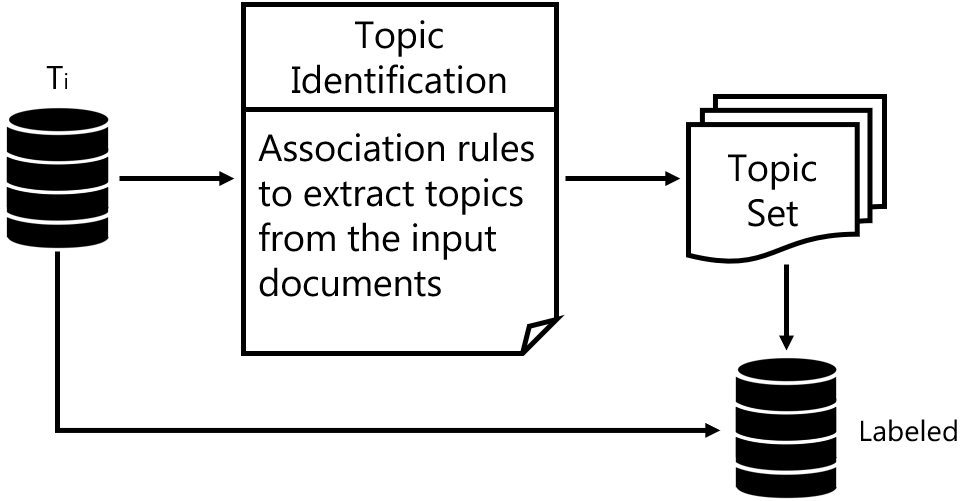
\includegraphics[width=0.8\linewidth]{01.Chapters/04.Materials/topic-identification}
	\caption{Topic identification process.}
	\label{fig:topic-identification}
\end{figure}

To perform this, in the first place, we need to make a few adjustments to our data by choosing the proper vocabulary. We already cut off some well-known stop words, like articles, adverbs, and conjunctions. However, there are still some words outside the conventional stop word lists that can disturb the performance of the NLP algorithms. Thus, from Zipf's law, we will apply a Luhn's cut
%, like proposed in Figure \ref{fig:zipfs-law-and-luhns-proposed-cut-off-points}, 
to eliminate both the most frequent and the least frequent words.

%\begin{figure}[h!]
%	\centering
%	% TODO: acho que vale a pena gerar sua figura aqui
%	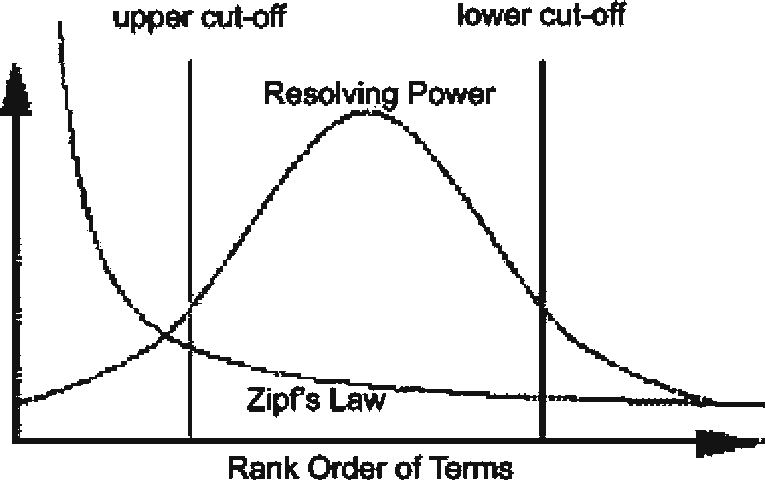
\includegraphics[width=0.55\linewidth]{01.Chapters/04.Materials/Zipfs-law-and-Luhns-proposed-cut-off-points}
%	\caption{Zipf’s law and Luhn’s proposed cut-off points, Figure from \cite{cummins2006evolving}.}
%	\label{fig:zipfs-law-and-luhns-proposed-cut-off-points}
%\end{figure}

After cutting off these words, we can finally advance to the topic modeling step. The LDA algorithm needs three parameters to execute, the Dirichlet distribution parameters $\alpha$ and $\beta$, and the numbers of topics $K$. To choose the best set we must run a hyperparameter optimization, on the \textit{Past} set, guided by the $C_{v}$ topic coherence metric.

Found the best parameters, we re-run the LDA on \textit{Past} set to fit the word distribution over topics and the topics distribution over documents. To label the data, we will proceed as follows, if for a topic the document has a probability greater than a certain threshold, we say the document has a positive class for that topic. So, at the end of this process, we will have for each $K$ topics a class to label the documents.

\subsection{Evaluating the \textit{Present}}\label{sec:material-combination}

In order to evaluate the ability for a model with the \textit{Past} make good predictions about the \textit{Present}, we must find some correspondence between the topics from both sets. We repeat the topic modeling on \textit{Present} set with their own vocabulary, after the Lunh's cut, by performing LDA with the same hyperparameters found by the optimization. Finally, we assign the found topics to the documents.

To associate the discovered topics from both data sets we will combine two techniques. The first one consists of comparing the intersection between the $N$ most likely words as described by:

\begin{equation}
	\label{eq:top-n-match}
	\text{Sim}_{1}\left(\text{Past}_{i}, \text{Present}_{j}\right) = \dfrac{|\text{Top}_{N}(\text{Past}_{i}) \cap \text{Top}_{N}(\text{Present}_{j})|}{N} \text{.}
\end{equation}

Where $\text{Top}_{N}(\text{Topic}_{k})$ represents the set of $N$ words with the higher probability to belong to $\text{Topic}_{k}$. Thus, the greater this score the greater the similarity between topics.

For the second technique, we need to represent the distribution of the words over topics only by the vocabularies intersection, so we measure the similarity by applying:

\begin{equation}
	\label{eq:global-match}
	\text{Sim}_{2}\left(\text{Past}_{i}, \text{Present}_{j}\right) = \sqrt{\sum_{v=1}^{V} \left(w_{v}^{\text{Past}_{i}} - w_{v}^{\text{Present}_{j}}\right)^2} \text{.}
\end{equation}

Where $V$ is the intersection vocabulary length and $w_{v}^{\text{Past}_{i}}$ represent the normalized probability for the $v^{\text{th}}$ word over the topic $\text{Past}_{i}$.

\section{Document Classification}

For each topic in our set of discovered topics, we must be able to identify which topics are covered by a new document. Thus, we will build a classifier to perform this verification. Knowing that a document can be about several topics, so we must have a multi-class classifier. We can see this as an individual binary classifier for each topic that tells us whether the document has it. Using the \textit{labeled Past} set it is possible to build this classifier. Figure \ref{fig:document-classification} illustrates it in detail.

\begin{figure}[h!]
	\centering
	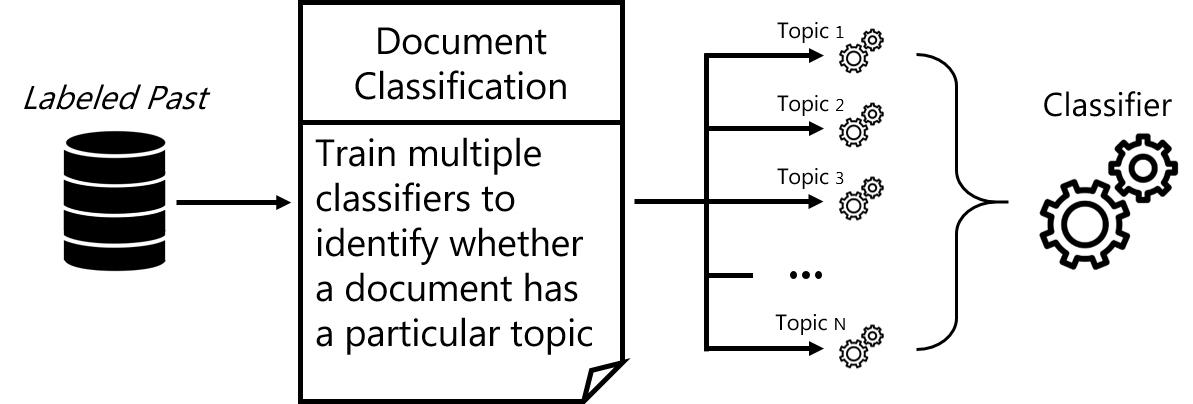
\includegraphics[width=0.9\linewidth]{01.Chapters/04.Materials/document-classification}
	\caption{Multi-class classifier from \textit{Labeled Past} set.}
	\label{fig:document-classification}
\end{figure}

Let us forget the multi-class problem for a while, let us focus in build a single classifier that predicts if a document talks about a certain topic. In this way, at the end of this process, we just repeat the training methods for all topics. With the \textit{Labeled Past} data set we will try different classification models with some vectorization techniques, like BoW, TF-IDF, and embedding methods. To evaluate the good fit for our models, we will perform cross-validation to evaluate the main metrics presented in section \ref{sub-sub:metrics}.

Chosen the best model for our data, we must study how these models, build from the past, behave in presence of present data. For this, we encode the \textit{Present} documents with the past vocabulary to guarantee that only the words already known by the model are used to decide the topics. Thus, we use these predictions in combination with the main topic correspondence to proceed with the analysis.

\section{Tools}

The source code for this work was done mainly with Python 3.8, \cite{python}. This language has support for several machine learning libraries that will facilitate the code's implementation. Let us briefly describe some of the main packages used so far.

The pre-processing pipeline requested lots of packages, the \textit{re} to apply regex cleaning methods, \textit{unidecode} to convert some special characters, \textit{contractions} to expand the contractions, \textit{nltk} to extract the preliminary stop-words, and \textit{spacy} to perform the lemmatization. For the topic modeling, we used mostly the \textit{gensim} models package. It provides user-friendly methods to perform and evaluate the LDA algorithm. For the classification, it was used the \textit{scikit-learn} both to vectorize the data and to build the models. Besides this some other mode commons packages were used, such as \textit{pandas} and \textit{numpy}, to array manipulation, and \textit{plotly} to display quality visualizations.

%\subsection{Forecast evaluation}
%
%Finally, to evaluate the time series model is the last task to be accomplished. Following the flowchart shown in Figure \ref{fig:forecast}, first, we have to label the \textit{Modeler} and \textit{Validation} sets. Then, using labeled \textit{Identifier} and \textit{Modeler} we will build a topic incidence matrix over the time, to apply a forecaster process for those time series. With the labeled \textit{Validation} set we will perform an evaluation for our model and then make conclusions about it.
%
%\begin{figure}[h!]
%	\centering
%	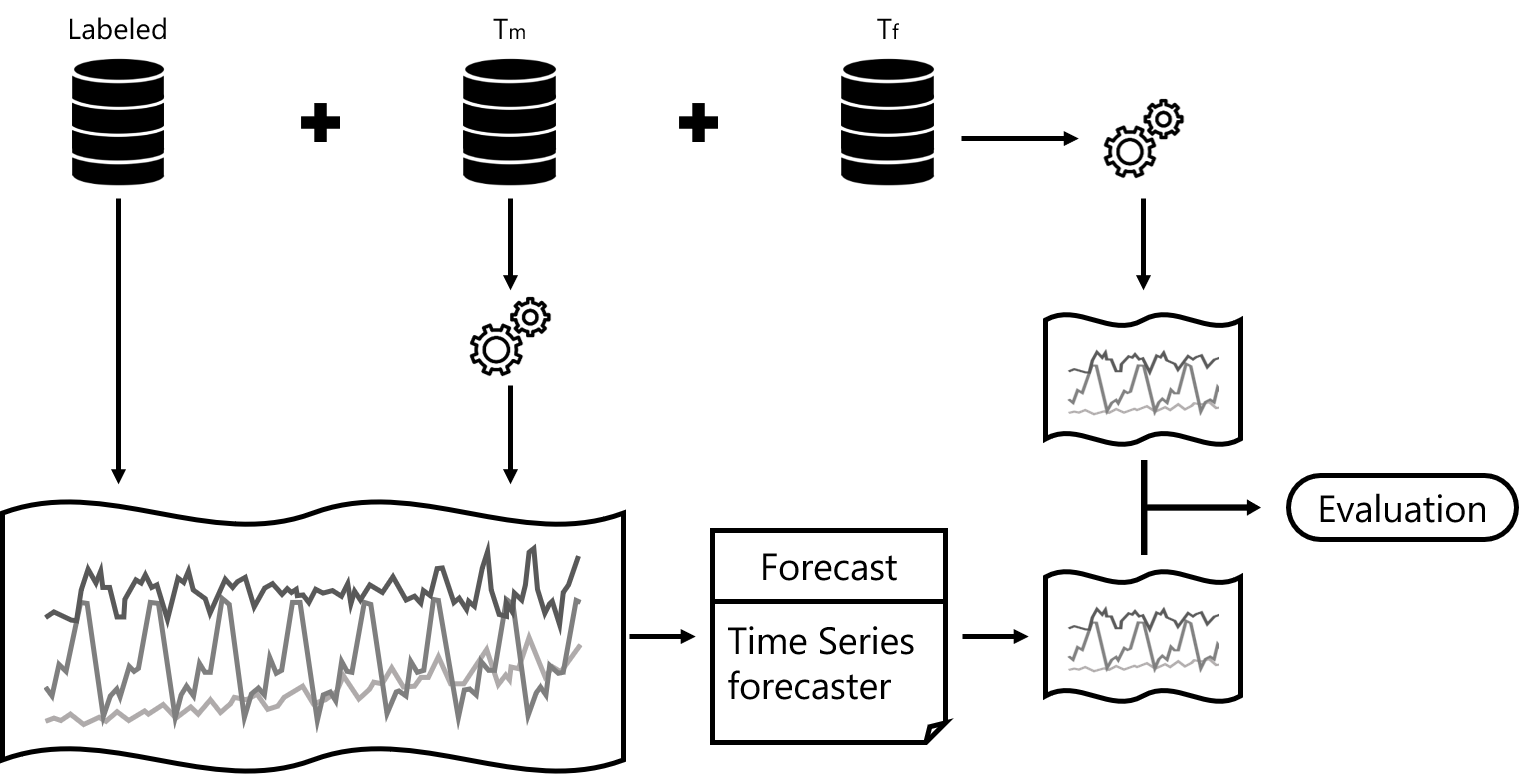
\includegraphics[width=\linewidth]{01.Chapters/04.Materials/forecast}
%	\caption{Flowchart to evaluate the time series model.}
%	\label{fig:forecast}
%\end{figure}

%As proposed we not going to dive too deep on the forecast evaluation, but we will provide a brief sneak peek from this step. Figure \label{fig:forecast-trucated} show the truncated step just with the formation of the incidence matrix.


\chapter{Results and Discussions}\label{chap:results}
In the last chapter, we detailed all the methodology steps behind the experimentation. In this one, we will show the proper results obtained by the topic modeling and classification steps.

\section{Topic Modeling}

In this first section, the results are related to the topic modeling step, divided into four stages: the vocabulary selection; the topic coherence optimization; applying LDA in past and present set; and the combination of topics from the past and future.

\subsection{Vocabulary Selection}

After the normalization, we had performed the Luhn's cut in order to remove words with document frequency higher than 60\% and words that appear in less than 5 documents. The cut was performed in both \textit{Past} and \textit{Present} sets, the Table \ref{tab:vocabulary} shows a brief description for the vocabularies dimension before and after the selection, and for their intersection.

\begin{table}[h!]
	\centering
	\caption{Vocabulary description.}
	\label{tab:vocabulary}
	\begin{tabular}{l|cccc}
		\toprule
		          &  \textbf{Raw}  & \textbf{High DF} & \textbf{Low DF} & \textbf{Filtered} \\ \midrule
		Past      & 77512 &   104   & 65480  &  11928   \\
		Present   & 90122 &   183   & 70356  &  19583   \\
		Intersect &   -   &    -    &   -    &   9745   \\ \bottomrule
	\end{tabular}
\end{table}

With this cut, words like ``abstract'', ``show'' and ``reference'' were removed from the vocabulary. They are quite common in this type of scientific publication and are not relevant for analysis. The low frequency includes very specific words and mostly misspellings.

\subsection{Topic Coherence Optimization}

To find the best topic model for our data, an hyperparameter optimization has been performed over the three LDA parameters: $\alpha \in \left\{0.1, 0.5, 1\right\}$, $\beta \in \left\{0.05, 0.1, 0.5, 1\right\}$ and $K \in \left\{10, 15, 20, 25, 30, 35, 40\right\}$. The dataset used was the \textit{Past} set with its vocabulary as described in the previous section. Figure \ref{fig:coherence-optimization} shows the coherence score $C_{\text{V}}$ by the number of topics for the main $\alpha$ and $\beta$ combinations.

\begin{figure}[h!]
	\begin{subfigure}{0.49\textwidth}
		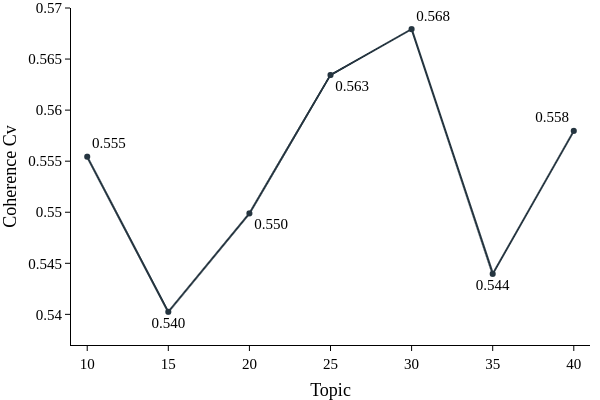
\includegraphics[width=\linewidth]{01.Chapters/05.Results/01_Topic_Cv_A:0.5| B:1.00}
		\caption{$\alpha = 0.5$ and $\beta = 1.0$.}
	\end{subfigure}%
	\hfill
	\begin{subfigure}{0.49\textwidth}
		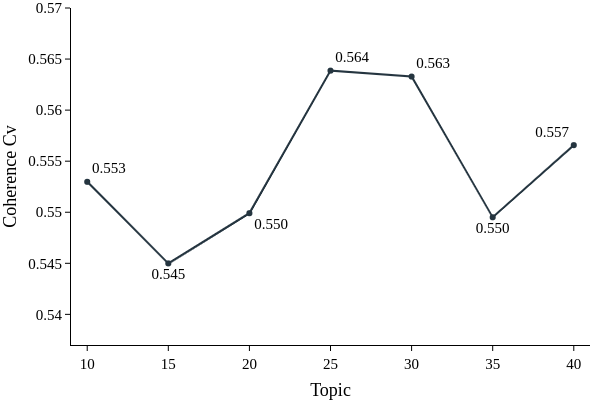
\includegraphics[width=\linewidth]{01.Chapters/05.Results/02_Topic_Cv_A:0.1| B:1.00}
		\caption{$\alpha = 0.1$ and $\beta = 1.0$.}
	\end{subfigure}%
	\vfill
	\begin{subfigure}{0.49\textwidth}
		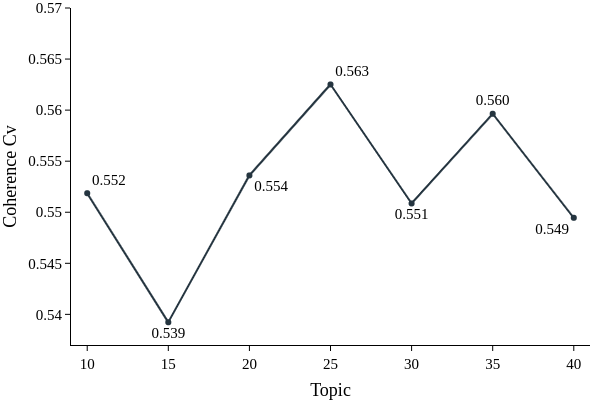
\includegraphics[width=\linewidth]{01.Chapters/05.Results/03_Topic_Cv_A:1.0| B:1.00}
		\caption{$\alpha = 1.0$ and $\beta = 1.0$.}
	\end{subfigure}%
	\hfill
	\begin{subfigure}{0.49\textwidth}
		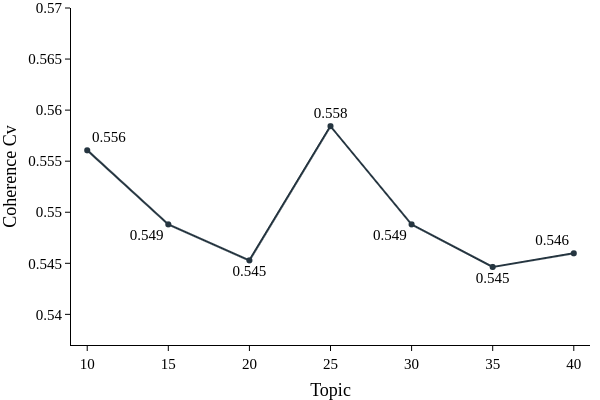
\includegraphics[width=\linewidth]{01.Chapters/05.Results/04_Topic_Cv_A:1.0| B:0.10}
		\caption{$\alpha = 1.0$ and $\beta = 0.1$.}
	\end{subfigure}%
	\caption{Topic Coherence Optimization.}
	\label{fig:coherence-optimization}
\end{figure}

Although the combination for $\alpha = 0.5$ and $\beta = 1.0$ has it maximum for $30$ topics, we can clearly detect a maximum trend for $25$ topics. From the application point of view, the smaller the number of topics the better for a human to follow their evolution. In this manner, we decided on $25$ topics to proceed with the experiment, with this value for $K$, the $\alpha$ and $\beta$ parameters with the best coherence score are $0.1$ and $1.0$, respectively.

\subsection{Finding Topics}

At this stage we had performed the LDA algorithm over the \textit{Past} and \textit{Present} sets, with the parameters established in the previous stage and their respective vocabularies, to find their topics. After the modeling the \textit{Present} model has presented a coherence of $0.614$, this indicates that the \textit{Present} model is slightly better than the \textit{Past} one.

\subsubsection{Past}

Figure \ref{fig:past-wordcloud} shows some word clouds for \textit{Past} topics that are easier to identify what they talk about. For example, topic 0 talks about image recognition, topic 10 clearly is about reinforcement learning, topic 16 can be about supervised learning, and topic 19 about facial recognition. To assess all the topics in more detail check Appendix \ref{apdx:past}.

\begin{figure}[h!]
	\begin{subfigure}{0.49\textwidth}
		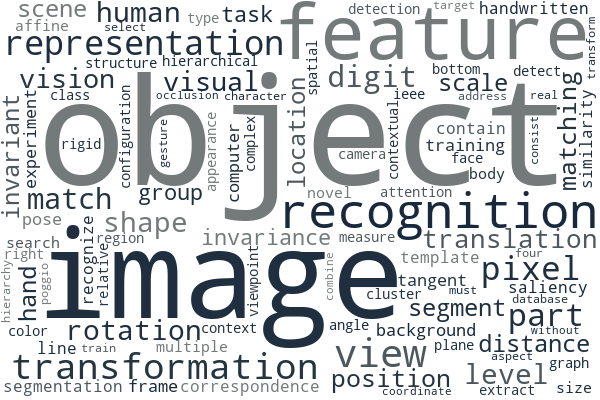
\includegraphics[width=\linewidth]{01.Chapters/05.Results/past_00}
		\caption{Past topic number 0.}
	\end{subfigure}%
	\hfill
	\begin{subfigure}{0.49\textwidth}
		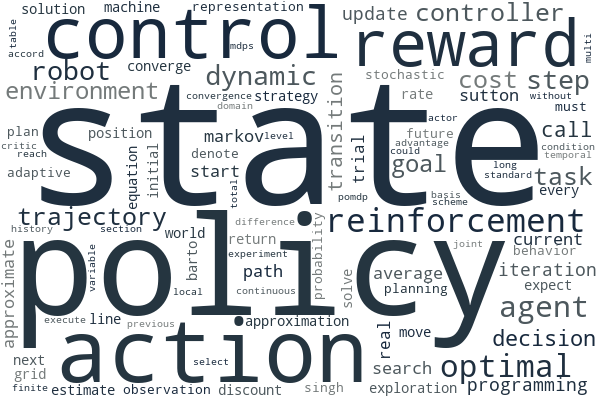
\includegraphics[width=\linewidth]{01.Chapters/05.Results/past_10}
		\caption{Past topic number 10.}
	\end{subfigure}%
	\vfill
	\begin{subfigure}{0.49\textwidth}
		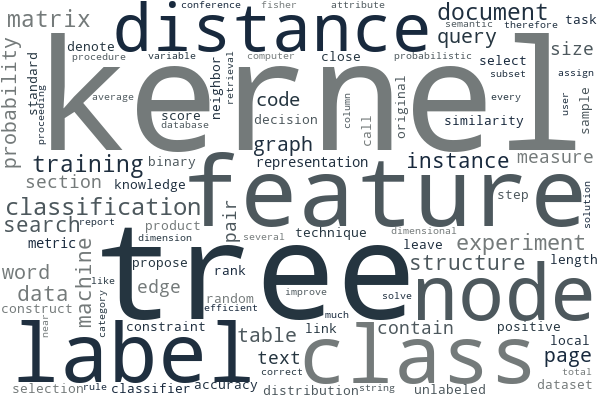
\includegraphics[width=\linewidth]{01.Chapters/05.Results/past_16}
		\caption{Past topic number 16.}
	\end{subfigure}%
	\hfill
	\begin{subfigure}{0.49\textwidth}
		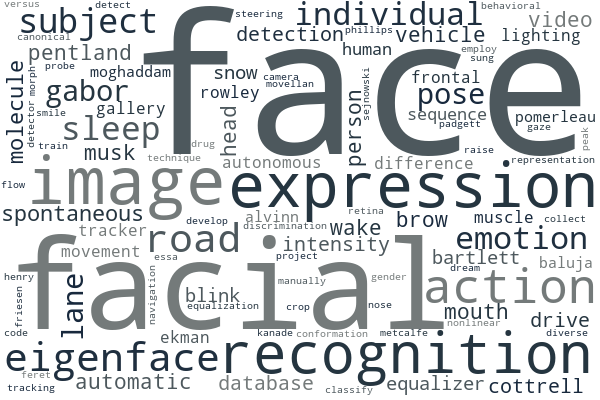
\includegraphics[width=\linewidth]{01.Chapters/05.Results/past_19}
		\caption{Past topic number 19.}
	\end{subfigure}%
	\caption{\textit{Past} topics wordclouds.}
	\label{fig:past-wordcloud}
\end{figure}

Besides getting the topics we also have the distribution of the documents of topics. Using these distributions we had labeled the documents as positive or negative for the topics with a threshold of $1 / K$, i.e., for a document covers a given topic his probability has to be at least $0.08$. This probability guarantees, by the pigeonhole principle, that the documents have at least one topic.

Figure \ref{fig:past-topic-dist} shows the distribution of topics over the documents. In Figure \ref{fig:past-percentage-bar} we have the percentage of documents that is about the 25 past topics, Figure \ref{fig:past-percentage-hist} shows the histogram for these percentages, each bin with $2.5\%$. According to the figures, none of the topics are in more than $50\%$ of the documents, some of them are present in less than $2.5\%$, but mostly they are distributed between $10\%$ and $35\%$.

\begin{figure}[h!]
	\begin{subfigure}{0.49\textwidth}
		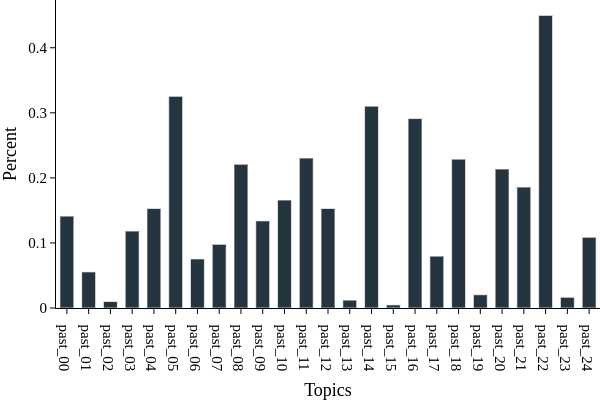
\includegraphics[width=\linewidth]{01.Chapters/05.Results/past-percentage-bar}
		\caption{Percentage of documents with topics.}
		\label{fig:past-percentage-bar}
	\end{subfigure}%
	\hfill
	\begin{subfigure}{0.49\textwidth}
		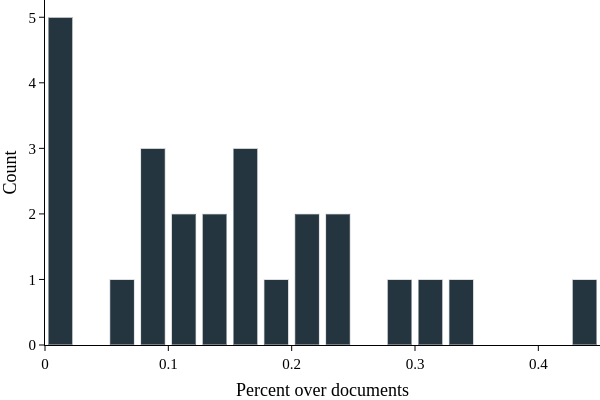
\includegraphics[width=\linewidth]{01.Chapters/05.Results/past-percentage-hist}
		\caption{Histogram for the topic percentages.}
		\label{fig:past-percentage-hist}
	\end{subfigure}%
	\caption{Distribution of topics over the documents.}
	\label{fig:past-topic-dist}
\end{figure}

Figure \ref{fig:past-topic-per-doc} shows the distribution of topics in each document. This histogram shows that most documents have more than one topic, a few have only one topic, even fewer have more than 7, and none document has more than 10 topics.

\begin{figure}[h!]
	\centering
	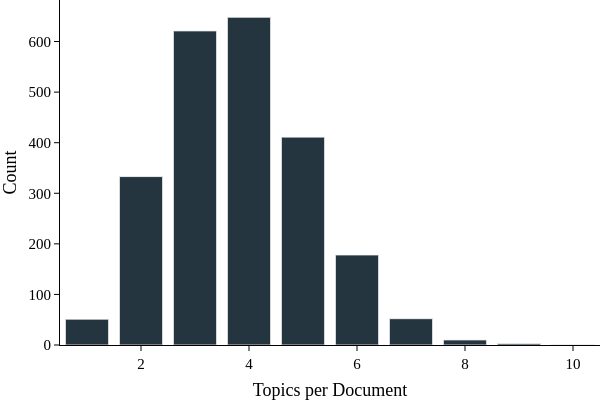
\includegraphics[width=0.6\linewidth]{01.Chapters/05.Results/past-topic-per-doc}
	\caption{Histogram for the number of topics per document.}
	\label{fig:past-topic-per-doc}
\end{figure}


\subsubsection{Present}

Figure \ref{fig:pres-wordcloud} shows some word clouds for \textit{Present} topics that are easier to identify what they talk. For example, topic 0 clearly is about NLP and topic modeling, topic 13 is about clustering, topic 16 can be about statistical inference, and topic 24 about classification. To access all the topics in more detail check Appendix \ref{apdx:present}.

\clearpage
\begin{figure}[h!]
	\begin{subfigure}{0.49\textwidth}
		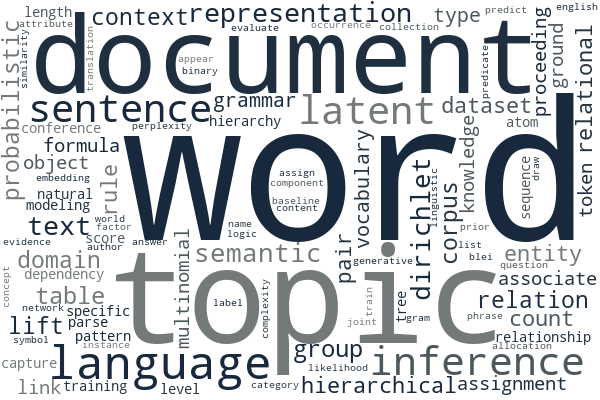
\includegraphics[width=\linewidth]{01.Chapters/05.Results/pres_00}
		\caption{Present topic number 0.}
	\end{subfigure}%
	\hfill
	\begin{subfigure}{0.49\textwidth}
		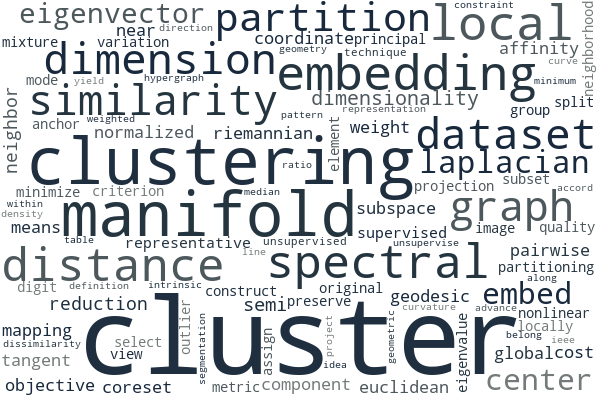
\includegraphics[width=\linewidth]{01.Chapters/05.Results/pres_13}
		\caption{Present topic number 13.}
	\end{subfigure}%
	\vfill
	\begin{subfigure}{0.49\textwidth}
		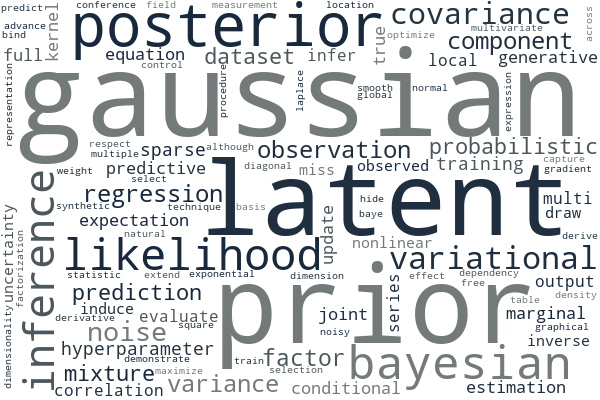
\includegraphics[width=\linewidth]{01.Chapters/05.Results/pres_16}
		\caption{Present topic number 16.}
	\end{subfigure}%
	\hfill
	\begin{subfigure}{0.49\textwidth}
		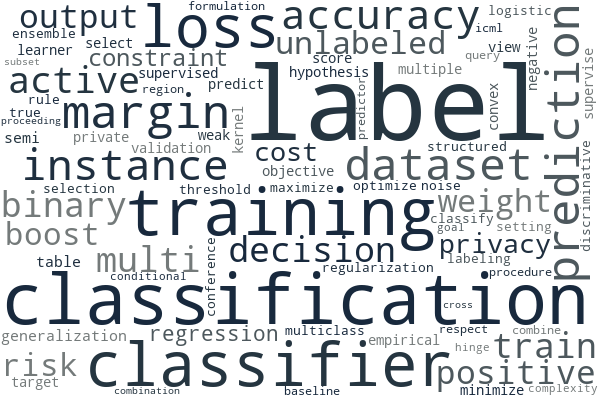
\includegraphics[width=\linewidth]{01.Chapters/05.Results/pres_24}
		\caption{Present topic number 24.}
	\end{subfigure}%
	\caption{\textit{Present} topics wordclouds.}
	\label{fig:pres-wordcloud}
\end{figure}

Figures \ref{fig:pres-topic-dist} and \ref{fig:pres-topic-per-doc} have the same idea as the Figures \ref{fig:past-topic-dist} and \ref{fig:past-topic-per-doc}. The \ref{fig:pres-topic-dist} shows that the topics are well distributed over the documents, the topic present in more documents is about $35\%$ of them. Figure \ref{fig:pres-topic-per-doc} shows the distribution of \textit{present} topics over the docuements, similarly to the \textit{past} distribution, the documents have mostly about 3 and 4 topics and none of then have more than 10 topics.

\begin{figure}[h!]
	\begin{subfigure}{0.49\textwidth}
		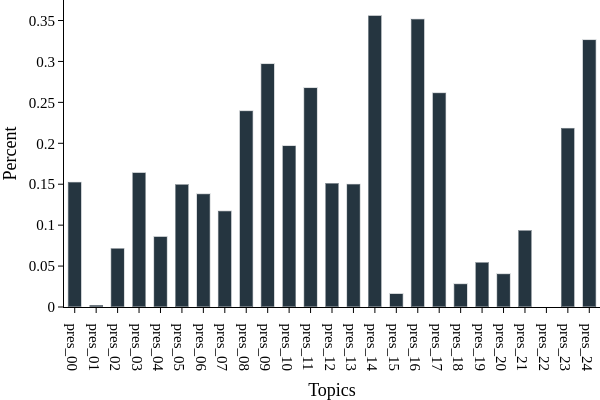
\includegraphics[width=\linewidth]{01.Chapters/05.Results/pres-percentage-bar}
		\caption{Percentage of documents with topics.}
		\label{fig:pres-percentage-bar}
	\end{subfigure}%
	\hfill
	\begin{subfigure}{0.49\textwidth}
		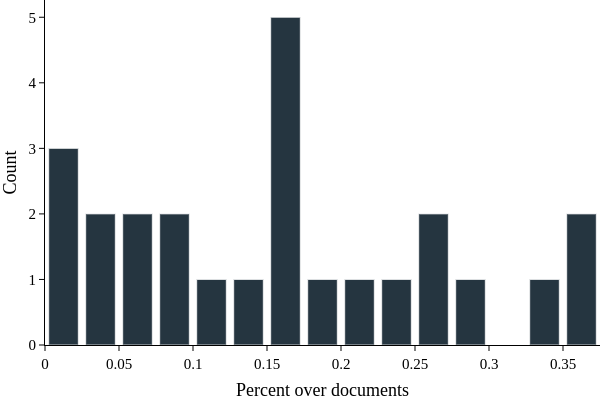
\includegraphics[width=\linewidth]{01.Chapters/05.Results/pres-percentage-hist}
		\caption{Histogram for the topic percentages.}
		\label{fig:pres-percentage-hist}
	\end{subfigure}%
	\caption{Distribution of topics over the documents.}
	\label{fig:pres-topic-dist}
\end{figure}

\begin{figure}[h!]
	\centering
	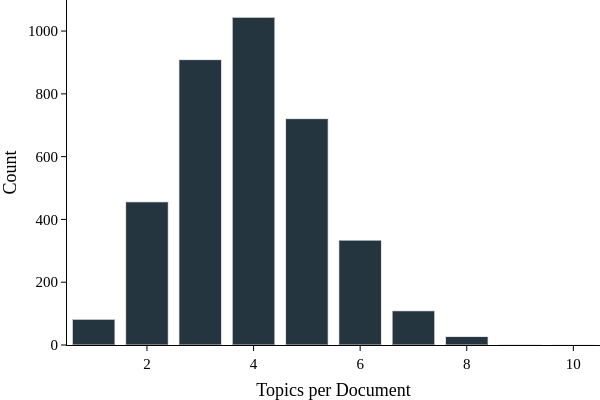
\includegraphics[width=0.55\linewidth]{01.Chapters/05.Results/pres-topic-per-doc}
	\caption{Histogram for the number of topics per document.}
	\label{fig:pres-topic-per-doc}
\end{figure}

\subsection{Past-Present Correspondence}

With the \textit{past} and \textit{present} topics defined, the similarity metrics described in section \ref{sec:material-combination} were applied to obtain the topic correspondence. For $\text{Sim}_{1}$, we use the top 50 words, i.e., $N=50$. As $\text{Sim}_{1}$ and $\text{Sim}_{2}$ are negatively correlated, to aggregate then, we divide $\text{Sim}_{1}$ for $\text{Sim}_{2}$ to capture the best from both metrics. Table \ref{tab:correspondence-score} illustrates the main correspondences between \textit{past} and \textit{present} topics.

\begin{table}[h!]
	\centering
	\caption{Main association for \textit{past} and \textit{present} topics.}
	\label{tab:correspondence-score}
	\begin{tabular}{cc|ccc}
		\toprule
		\textbf{Past} & \textbf{Present} & \textbf{$\text{Sim}_{1}$} & \textbf{$\text{Sim}_{2}$} & \textbf{$\text{Sim}_{1} / \text{Sim}_{2}$} \\ \midrule
		 11 &   06 &   58\% &   0.026 &   22.39 \\
		 10 &   05 &   56\% &   0.031 &   18.23 \\
		 14 &   16 &   44\% &   0.040 &   11.11 \\
		 20 &   09 &   38\% &   0.036 &   10.56 \\
		 18 &   11 &   40\% &   0.043 &    9.35 \\
		 07 &   12 &   34\% &   0.038 &    8.91 \\
		 04 &   02 &   54\% &   0.061 &    8.82 \\
		 00 &   08 &   46\% &   0.055 &    8.36 \\
		 05 &   03 &   32\% &   0.047 &    6.83 \\
		 22 &   07 &   36\% &   0.057 &    6.27 \\ \bottomrule
	\end{tabular}
\end{table}

By aggregating the two metrics, we are choosing topics whose common word distribution is similar while giving priority to topics with the most similar top words. For example, take the correspondence 18-11 and 07-12, the second one is the closest in terms of word distribution, but the first has the top 50 more similar making this correspondence stronger. Table \ref{tab:correspondence-words} shows the intersection for those top 10 topic correspondences.

\begin{table}[h!]
	\centering
	\caption{Words intersection for the main correspondence.}
	\label{tab:correspondence-words}
	\begin{tabular}{cc|lllll}
		\toprule
		\textbf{Present} & \textbf{Past} & \multicolumn{5}{c}{\textbf{Words}} \\ \midrule
		11 & 06 & neuron   & spike      & cell        & response   & stimulus      \\
		10 & 05 & policy   & action     & control     & reward     & reinforcement \\
		14 & 16 & gaussian & mixture    & likelihood  & prior      & bayesian      \\
		20 & 09 & gradient & constraint & convergence & update     & cost          \\
		18 & 11 & bound    & theorem    & loss        & bind       & proof         \\
		07 & 12 & subject  & stimulus   & human       & response   & trial         \\
		04 & 02 & signal   & filter     & noise       & frequency  & channel       \\
		00 & 08 & object   & image      & recognition & pixel      & shape         \\
		05 & 03 & markov   & inference  & sequence    & likelihood & bayesian      \\
		22 & 07 & unit     & training   & layer       & train      & hide          \\ \bottomrule
	\end{tabular}
\end{table}

Through the intersections we see that some \textit{past} topics continued in the \textit{present}. For example, the correspondence 10-05 talks about reinforcement learning, and 22-07 is about deep learning. From that, we evaluate how the models of the \textit{past} behave with the \textit{present}.

\section{Document Classification}

This section will cover the results behind the classification model. First, the training process and model selection with the \textit{Past} set, then, the evaluation of those models at \textit{Present} according to the combination of topics.

\subsection{Model Selection}

%With the documents labeled, we now have our \textit{Labeled Past} dataset. From that, we can train a binary classification model for each topic. For the classification was performed cross-validation with 10 folds for each combination of vectorization + model, the raw results for those models are in Appendix \ref{apdx:classification}.

We now have the \textit{Labeled Past} dataset. From that, we can train a classification model for each topic. For this was performed cross-validation with 10 folds for each combination of vectorization + model, the raw results for those models are in Appendix \ref{apdx:classification}.

%To evaluate which model is the best, we will compare the average of the model scores for all topics. Table \ref{tab:classification-report} shows the comparison between the precision, recall and f1 score for the models. As marked in the table, the best model is the XXXX with XXXX.

To evaluate which model is the best, we will compare the average of the model scores for all topics. 
So for each combination of vectorization + model, we apply an arithmetic average for all individual classifiers metrics to compare and choose the best combination.
Table \ref{tab:classification-report} shows the comparison between the precision, recall, and f1 for the models.
As marked in the table, the best model is the TF-IDF with SVM.

\begin{table}[h!]
	\centering
	\caption{Classification models comparison.}
	\label{tab:classification-report}
	\begin{tabular}{c|ccc}
		\toprule
		\multirow{2}{*}{\textbf{Type}} & \multicolumn{3}{c}{\textbf{Statistics}} \\\cmidrule{2-4}
		 & \textbf{Precision} & \textbf{Recall} & \textbf{F1 Score} \\ \midrule
		\multicolumn{1}{l|}{BOW + Naive Bayes}     & 0.656 & 0.781 & 0.695 \\
		\multicolumn{1}{l|}{TF-IDF + Naive Bayes}  & 0.719 & 0.483 & 0.553 \\
		\multicolumn{1}{l|}{BOW + SVM}             & 0.863 & 0.539 & 0.648 \\
		\multicolumn{1}{l|}{\textbf{TF-IDF + SVM}} & \textbf{0.906} & \textbf{0.683} & \textbf{0.769} \\
%		\multicolumn{1}{l|}{GloVe + SVM}        & - & - & - \\
		\bottomrule
	\end{tabular}
\end{table}

Following these results, we identified that we have a bias for higher precision than recall. These results show us the models tend not to predict more positive classes than the existent ones, on the other hand, the smaller recall indicates the models are mispredicting the documents that really belongs to that class. Tables \ref{tab:nb-bow} to \ref{tab:svm-tfidf}, from Appendix \ref{apdx:classification}, also show the more imbalanced the class, the predictions tend to be less accurate.


\subsection{Evaluating Present Predictions}

With the built classifiers from the \textit{Labeled Past} set, we apply it in the \textit{present} set and compare the output with its labels. Using just the top-10 correspondences in Table \ref{tab:correspondence-score} we have obtained the average results for this predictions shown in Table \ref{tab:avg-combination-score} below.

\begin{table}[h!]
	\centering
	\caption{Metrics for the top-10 topic combinations.}
	\label{tab:avg-combination-score}
	\begin{tabular}{cc|ccc}
		\toprule
		\textbf{Past} & \textbf{Present} & \textbf{Precision} & \textbf{Recall} & \textbf{F1 Score} \\ \midrule
		11 & 06 & 0.976 & 0.563 & 0.714 \\
		10 & 05 & 0.936 & 0.709 & 0.807 \\
		14 & 16 & 0.640 & 0.697 & 0.667 \\
		20 & 09 & 0.699 & 0.547 & 0.614 \\
		18 & 11 & 0.552 & 0.795 & 0.651 \\
		07 & 12 & 0.790 & 0.249 & 0.379 \\
		04 & 02 & 0.454 & 0.355 & 0.398 \\
		00 & 08 & 0.967 & 0.368 & 0.533 \\
		05 & 03 & 0.324 & 0.820 & 0.464 \\
		22 & 07 & 0.680 & 0.550 & 0.608 \\
		\bottomrule
	\end{tabular}
\end{table}

In addition to this comparison, we want to evaluate the behavior of the models over the years. For this, we will evaluate the f1 score for each year isolated. In Figure \ref{fig:f1-combination} is presented the charts for them over the years, Figure \ref{fig:top1-5} shows the first to fifth, and Figure \ref{fig:top6-10} shows the remaining correspondences.

\begin{figure}[h!]
	\begin{subfigure}{0.49\textwidth}
		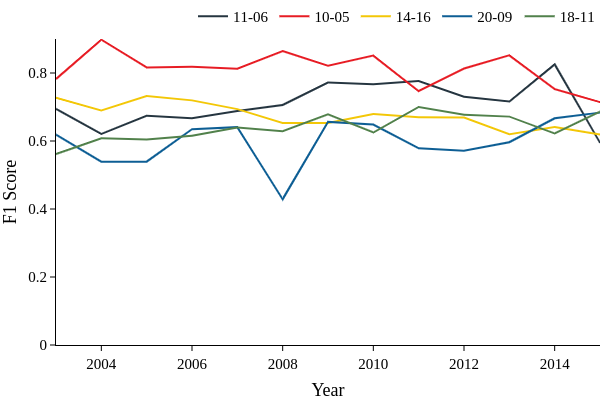
\includegraphics[width=\linewidth]{01.Chapters/05.Results/f1-combination-1-5}
		\caption{Correspondences 1 to 5.}
		\label{fig:top1-5}
	\end{subfigure}%
	\hfill
	\begin{subfigure}{0.49\textwidth}
		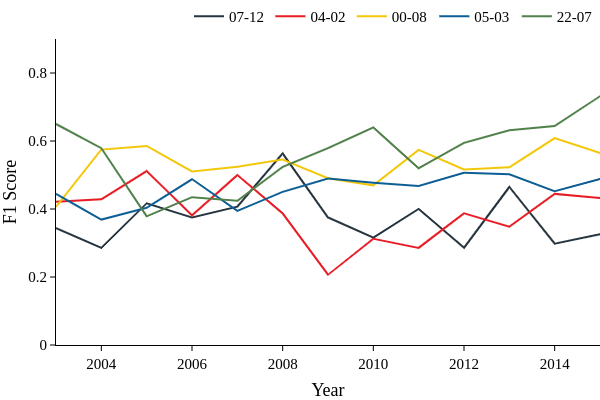
\includegraphics[width=\linewidth]{01.Chapters/05.Results/f1-combination-6-10}
		\caption{Correspondences 6 to 10.}
		\label{fig:top6-10}
	\end{subfigure}%
	\caption{F1 Score for the main correspondences.}
	\label{fig:f1-combination}
\end{figure}


% Comentar resultados das tabelas e dos gráficos
From Table \ref{tab:avg-combination-score}, we see a high negative correlation between the position of correspondences and their f1 scores, $-0.775$ for the record. This result said to us that is a decreasing relationship between the predictions of these correspondences. Figure \ref{fig:combination-corr} shows a scatter plot for this relationship with an ordinary least squares (OLS) trend line.

\begin{figure}[h!]
	\centering
	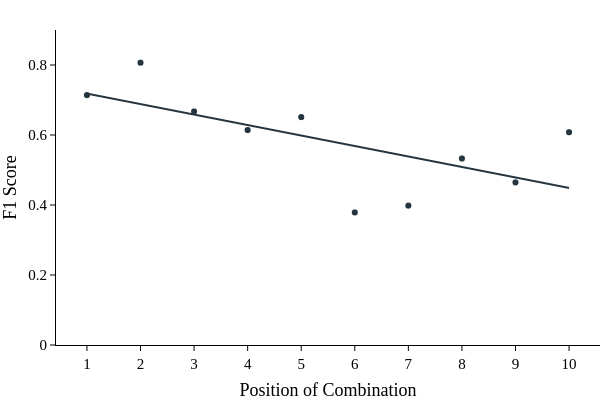
\includegraphics[width=0.6\linewidth]{01.Chapters/05.Results/combination-corr}
	\caption{F1 Score correlation with the correspondence position.}
	\label{fig:combination-corr}
\end{figure}

This decreasing trend reflects directly in score curves in Figure \ref{fig:f1-combination}. Despite slight fluctuations, the decreasing trend in correspondences scores could indicate that even in the best correspondences the predictions are not so accurate. The terms evolution over the years to develop the topics maybe have changed and the models can not learn these new terms.

Let us observe a little deeper at the relationship between the score and the time evolution. In Figure \ref{fig:isolated-topics} we have a scatter plot with the local regression trendline of LOWESS type for the two best correspondences. Notice that despite a small increase, there is a natural tendency of constancy followed by a decrease in the models' efficiency over the years. Again, this inclination suggests that the rising of new terms for new techniques affects the classification.

\begin{figure}[h!]
	\begin{subfigure}{0.5\textwidth}
	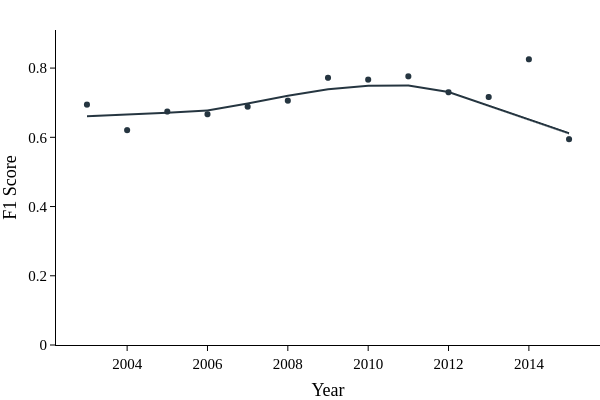
\includegraphics[width=\linewidth]{01.Chapters/05.Results/lowess-1}
		\caption{Topics correspondence \textit{Past 11} - \textit{Present 06}.}
	\end{subfigure}%
	\hfill
	\begin{subfigure}{0.5\textwidth}
		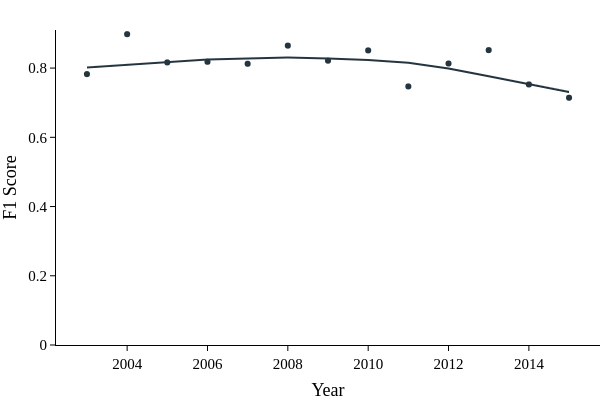
\includegraphics[width=\linewidth]{01.Chapters/05.Results/lowess-2}
		\caption{Topics correspondence \textit{Past 10} - \textit{Present 05}.}
	\end{subfigure}%
	\caption{F1 Score for the main correspondences.}
	\label{fig:isolated-topics}
\end{figure}

\newpage
Realize that correspondences under the top 5 may have some growth trend. However, in general, these correspondences already have low efficiency in relation to the best ones, decreasing the result's reliability.




\chapter{Conclusions, Recommendations, and Future Works}\label{chap:conclusion}
In this last chapter, we wrap up this work sharing conclusions. We also suggest new research lines inspired by the results of this work.

\section{Conclusions}

The main goal of this work was to evaluate the ability of classification models built from the topic modeling data, obtained by Latent Dirichelt Allocation. With a subset of documents, initial on time, called by \textit{Past}, we obtained their natural topics, then we do the same for intermediate data, called by \textit{Present}. After discovering the best combinations for these topics, we built classification models for each one of them and evaluate the predictions over the years.

In the chapter \ref{chap:intro}, we show a brief introduction, presenting the motivation and objective of this work. In chapter \ref{chap:literature} we described some important concepts of Natural Processing Language and classification techniques. In chapter \ref{chap:related} we presented related works that implement steps used in this work. 

Chapter \ref{chap:materials} described the whole methodology used to conduct the experimentation in this work, describing carefully each individual step. Finally, \ref{chap:results} presented and discussed the results obtained in each step of the experiment.

In synthesis, we saw from the results that is really possible to classify documents in short term, from a little subset of data. However, the topics evolve as time goes forward, evidenced by the discrepancy between the main closest combinations and those that follow right away.

We identified two aspects for these classification models. Firstly, we have a tendency of constancy in the efficiency of the model, because of the slow evolution of a given subject, mostly when dealing with scientific publications, as in our case. The second aspect shows a decreasing trend over time, as the model tends to unlearn about themes as new terms are used, such as neural networks, for example, recently the use of deep learning for these kinds of applications has become very popular.

Given this decreasing aspect, our models gradually lose their ability to predict. Therefore, a re-train routine could be fundamental to always keep achieving good results.

\section{Future Work}

From now, we propose other research lines some improvements directly by the results previously obtained:

\begin{itemize}
	\item \textit{Forecast Step:}
	
	The immediate continuation given the chronological order is develop the forecast step. Following the flowchart shown in Figure \ref{fig:forecast}, first, using the classifier we can build the incidence topic incidence matrix over time, with \textit{Past} and \textit{Present} sets. Then, apply a forecaster process for those time series with a Long Short-Term Memory neural network \cite{hochreiter1997long}. Finally, with the \textit{Future} set, perform an evaluation for the built forecaster.
	
	\begin{figure}[h!]
		\centering
		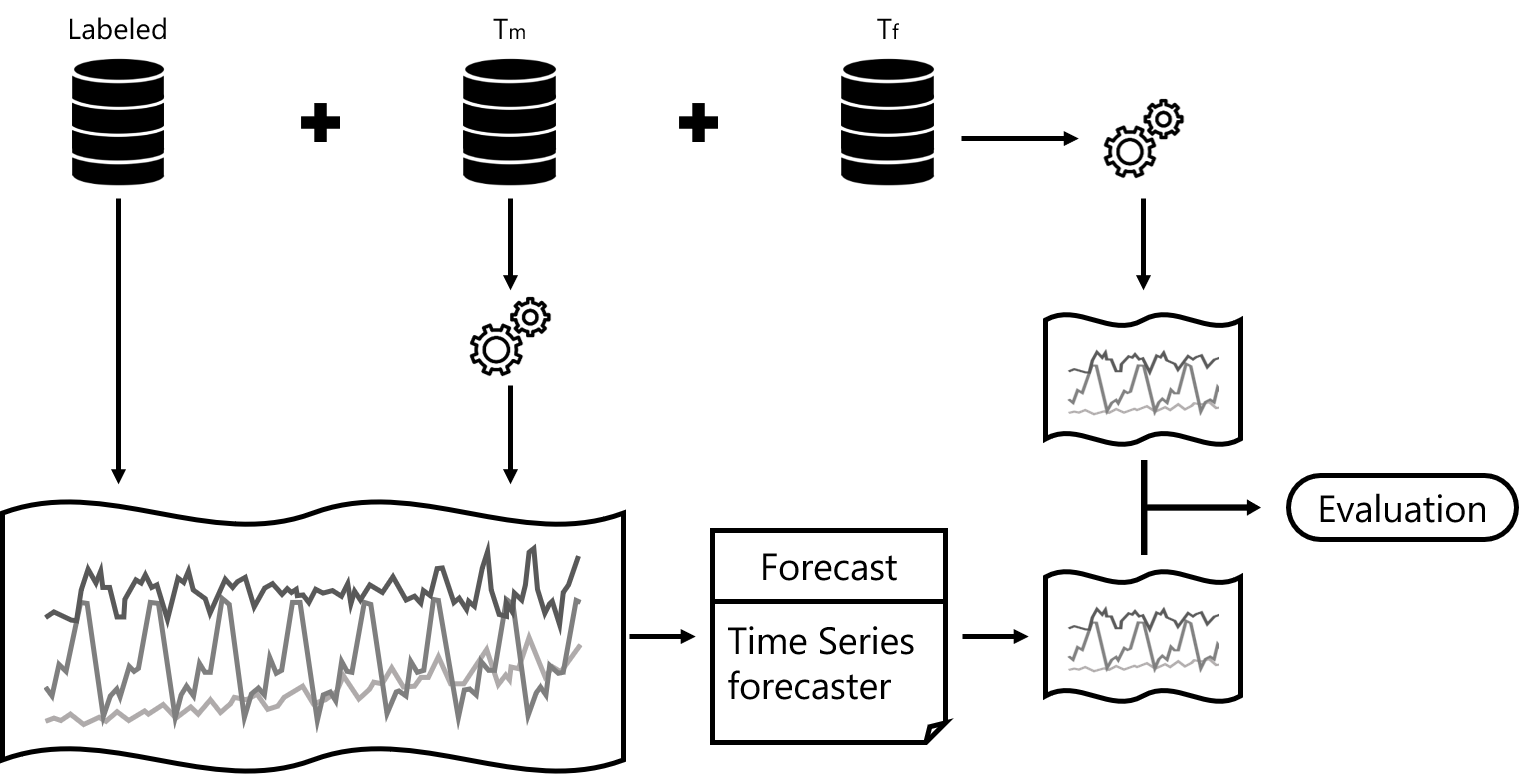
\includegraphics[width=0.8\linewidth]{01.Chapters/04.Materials/forecast}
		\caption{Flowchart to evaluate the time series model.}
		\label{fig:forecast}
	\end{figure}
	
	\item \textit{Retraining point:}
	
	Seeking to use this forecasting famework in a production enviroment, we will need to reduce the time granularity to month or even days. But, as we saw in Figure \ref{fig:isolated-topics} the classification models are losing efficiency over time. This research line aims to propose and evaluate metrics to identify an optimal threshold for retraining the topic model in order to uptade them with the new terms.
	
%	\item \textit{Topic modeling based on context:}
	
%	Text clusteing

	\item \textit{Feature extraction improvement:}
	
	In section \ref{sec:text-processing} we saw many techniques for normalization and vectorizing, but it doesn't stop there. There are several unexplored techniques that can improve our topic models and classification such as n-grams, hashing vectorizer and polinomial features, the word embedding itself presented a bad result due to the lack of a pre-trained model based on scientific publication context. This research line aims to use more sophisticated techniques for improve the topic and classification models, 
	
	
\end{itemize}


%\chapter{Roadmap}\label{chap:roadmap}
%Because of the problem's complexity, we can elaborate on a schedule with the proposed tasks in the previous chapter. Starting from August 3rd until November 9th we have 14 weeks, so we can divide the work into 6 sprints, 4 of them with 2 weeks, and the remainder two with 3 weeks. The Table \ref{tab:roadmap-table} show the tasks over the remaining months until the end of this work.

\begin{table}[h!]
	\centering
	\caption{Tasks schedule over the months.}
	\label{tab:roadmap-table}
	\begin{tabular}{c|cccl}
		\hline
		       \textbf{Sprint}        &    \textbf{Start Date}     &       \textbf{End Date}       &  \textbf{Duration}  & \textbf{Task}                     \\ \hline
		\multirow{2}{*}{\textbf{\#1}} & \multirow{2}{*}{August 3}  &  \multirow{2}{*}{August 16}   & \multirow{2}{*}{14} & - Chose a database                \\
		                              &                            &                               &                     & - Pre process the database        \\ \hline
		        \textbf{\#2}          &         August 17          &           August 30           &         14          & - Topic Identification            \\ \hline
		\multirow{2}{*}{\textbf{\#3}} & \multirow{2}{*}{August 31} & \multirow{2}{*}{September 20} & \multirow{2}{*}{21} & - Evaluate Identification         \\
		                              &                            &                               &                     & - Generate Identification Results \\ \hline
		        \textbf{\#4}          &        September 21        &           October 4           &         14          & - Document Classification         \\ \hline
		\multirow{2}{*}{\textbf{\#5}} & \multirow{2}{*}{October 5} &  \multirow{2}{*}{October 25}  & \multirow{2}{*}{21} & - Evaluate Classification         \\ 
		                              &                            &                               &                     & - Generate Classification Results \\ \hline
		        \textbf{\#6}          &         October 26         &          November 8           &         14          & - Test and fix bugs               \\ \hline
	\end{tabular}
\end{table}

In the table, we see that the forecasting step was not included in the schedule. Due to the high complexity of each stage, for this work, it will be implemented only up to the stage of the classification model. The last stage, with the forecast, will be for future work


% REFERENCIAS BIBLIOGRAFICAS
\renewcommand\bibname{\itareferencesnamebabel} %renomear título do capítulo referências
\bibliography{02.Referencias/referencias}

\setcounter{chapter}{0}

% Apendices
\appendix
\chapter{Past Topics}\label{apdx:past}
%{p{0.165\textwidth}p{0.165\textwidth}p{0.165\textwidth}p{0.165\textwidth}p{0.165\textwidth}}
%		\midrule \multicolumn{1}{|c|}{\textbf{First column}} & \multicolumn{1}{c|}{\textbf{Second column}} & \multicolumn{1}{c|}{\textbf{Third column}} \\ \midrule 
%		\endfirsthead
%		
%		\multicolumn{3}{c}%
%		{{\bfseries \tablename\ \thetable{} -- continued from previous page}} \\
%		\midrule \multicolumn{1}{|c|}{\textbf{First column}} & \multicolumn{1}{c|}{\textbf{Second column}} & \multicolumn{1}{c|}{\textbf{Third column}} \\ \midrule 
%		\endhead
%		
%		\midrule \multicolumn{3}{|r|}{{Continued on next page}} \\ \midrule
%		\endfoot
%		
%		\midrule \midrule
%		\endlastfoot

Table \ref{tab:past-topics} contains the top 10 words for the 25 topics obtained from the LDA algorithm in the \textit{Past} dataset.


\begin{center}
\begin{longtable}{
		>{\centering\arraybackslash}p{0.165\textwidth}
		>{\centering\arraybackslash}p{0.165\textwidth}
		>{\centering\arraybackslash}p{0.165\textwidth}
		>{\centering\arraybackslash}p{0.165\textwidth}
		>{\centering\arraybackslash}p{0.165\textwidth}}
	\caption{Top 10 words for the \textit{Past} topics.} \label{tab:past-topics} \\		
	\hline
	\textbf{Topic 00} & \textbf{Topic 01} & \textbf{Topic 02} & \textbf{Topic 03} & \textbf{Topic 04} \\ \hline
	     object       &      memory       &    hippocampus    &      circuit      & signal            \\
	      image       &     capacity      &    hippocampal    &       chip        & filter            \\
	     feature      &    associative    &   conditioning    &      analog       & motion            \\
	   recognition    &       store       &      episode      &      current      & noise             \\
	      view        &  representation   &      animal       &      voltage      & frequency         \\
	 transformation   &      recall       &      lesion       &      neuron       & channel           \\
	 representation   &       item        &      replay       &       vlsi        & temporal          \\
	      pixel       &      storage      &    neocortical    &       gate        & velocity          \\
	      part        &     retrieval     &   consolidation   &     implement     & visual            \\
	      digit       &       bind        &       dayan       &  implementation   & video             \\ \hline
	                  &                   &                   &                   &                   \\ \hline
	\textbf{Topic 05} & \textbf{Topic 06} & \textbf{Topic 07} & \textbf{Topic 08} & \textbf{Topic 09} \\ \hline
	   probability    &      cluster      &      subject      &       image       & classifier        \\
	  distribution    &     language      &     stimulus      &     component     & classification    \\
	      state       &      grammar      &     auditory      &      matrix       & class             \\
	    variable      &    clustering     &       human       &       pixel       & training          \\
	    estimate      &       rule        &     response      &       local       & feature           \\
	     markov       &       parse       &       trial       &    dimensional    & rate              \\
	     belief       &     structure     &       sound       &      feature      & detection         \\
	    inference     &     sentence      &       user        &       basis       & decision          \\
	  approximation   &      symbol       &      target       &  representation   & train             \\
	     sample       &      string       &       task        &      natural      & classify          \\ \hline
	                  &                   &                   &                   &                   \\
					  &                   &                   &                   &                   \\
					  &                   &                   &                   &                   \\
					  &                   &                   &                   &                   \\
	                  &                   &                   &                   &                   \\ \hline
	\textbf{Topic 10} & \textbf{Topic 11} & \textbf{Topic 12} & \textbf{Topic 13} & \textbf{Topic 14} \\ \hline
	      state       &      neuron       &       field       &    instruction    & gaussian          \\
	     policy       &       spike       &      visual       &      program      & mixture           \\
	     action       &       cell        &       cell        &     processor     & estimate          \\
	     control      &     response      &     direction     &       block       & distribution      \\
	     reward       &     stimulus      &     receptive     &     schedule      & sample            \\
	  reinforcement   &     synaptic      &    orientation    &     execution     & density           \\
	     optimal      &       rate        &      spatial      &      schema       & likelihood        \\
	      agent       &     activity      &     position      &      rollout      & data              \\
	      robot       &      firing       &     location      &     parallel      & prior             \\
	     dynamic      &     cortical      &      center       &       simd        & bayesian          \\ \hline
	                  &                   &                   &                   &                   \\ \hline
	\textbf{Topic 15} & \textbf{Topic 16} & \textbf{Topic 17} & \textbf{Topic 18} & \textbf{Topic 19} \\ \hline
	     packet       &      kernel       &       motor       &       bound       & face              \\
	      route       &       tree        &     movement      &      theorem      & facial            \\
	      load        &      feature      &      control      &      margin       & image             \\
	     traffic      &       label       &    oscillator     &       loss        & expression        \\
	      send        &       class       &     feedback      &       bind        & recognition       \\
	      slot        &       node        &       phase       &       class       & action            \\
	     routing      &     distance      &    trajectory     &       proof       & eigenface         \\
	      queue       &  classification   &      muscle       &      machine      & road              \\
	     router       &     document      &       axon        &  generalization   & subject           \\
	     switch       &     training      &     velocity      &     training      & sleep             \\ \hline
	                  &                   &                   &                   &                   \\ \hline
	\textbf{Topic 20} & \textbf{Topic 21} & \textbf{Topic 22} & \textbf{Topic 23} & \textbf{Topic 24} \\ \hline
	    gradient      &      dynamic      &       unit        &       game        & speech            \\
	    solution      &     equation      &     training      &      player       & word              \\
	   constraint     &       state       &       layer       &      protein      & recognition       \\
	     matrix       &       field       &       train       &       play        & speaker           \\
	  optimization    &     attractor     &       hide        &       gene        & training          \\
	   convergence    &     solution      &       task        &    equilibrium    & feature           \\
	     update       &      theory       &   architecture    &       nash        & state             \\
	     energy       &       line        &       node        &     strategy      & character         \\
	    equation      &      neuron       &      hidden       &     structure     & sequence          \\
	    minimize      &       limit       &    activation     &     sequence      & train             \\ \hline
\end{longtable}
\end{center}

\appendix
\chapter{Present Topics}\label{apdx:present}
Table \ref{tab:pres-topics} contains the top 10 words for the 25 topics obtained from the LDA algorithm in the \textit{Present} dataset.

\begin{center}
\begin{longtable}{
		>{\centering\arraybackslash}p{0.165\textwidth}
		>{\centering\arraybackslash}p{0.165\textwidth}
		>{\centering\arraybackslash}p{0.165\textwidth}
		>{\centering\arraybackslash}p{0.165\textwidth}
		>{\centering\arraybackslash}p{0.165\textwidth}}
	\caption{Top 10 words for the \textit{Present} topics.} \label{tab:pres-topics} \\		
	\hline
	\textbf{Topic 00} & \textbf{Topic 01} & \textbf{Topic 02} & \textbf{Topic 03} & \textbf{Topic 04} \\ \hline
	word              & wasserstein       & signal            & sampling          & rank              \\
	topic             & orbit             & source            & chain             & item              \\
	document          & transport         & event             & markov            & user              \\
	language          & lattice           & frequency         & inference         & query             \\
	inference         & conical           & speech            & gibb              & ranking           \\
	latent            & sinkhorn          & sensor            & posterior         & permutation       \\
	sentence          & simplicial        & speaker           & sampler           & preference        \\
	representation    & cone              & noise             & mcmc              & score             \\
	text              & cuturi            & audio             & particle          & worker            \\
	dirichlet         & barycenter        & channel           & carlo             & rating            \\ \hline
	                  &                   &                   &                   &                   \\ \hline
	\textbf{Topic 05} & \textbf{Topic 06} & \textbf{Topic 07} & \textbf{Topic 08} & \textbf{Topic 09} \\ \hline
	policy            & neuron            & network           & image             & gradient          \\
	action            & spike             & layer             & object            & update            \\
	reward            & network           & deep              & pixel             & iteration         \\
	agent             & cell              & training          & detection         & convergence       \\
	game              & stimulus          & train             & segmentation      & stochastic        \\
	control           & activity          & unit              & recognition       & constraint        \\
	trajectory        & population        & output            & patch             & objective         \\
	player            & response          & convolutional     & visual            & convex            \\
	dynamic           & dynamic           & architecture      & scene             & descent           \\
	reinforcement     & synaptic          & representation    & face              & message           \\ \hline
	                  &                   &                   &                   &                   \\
					  &                   &                   &                   &                   \\
					  &                   &                   &                   &                   \\
					  &                   &                   &                   &                   \\
	                  &                   &                   &                   &                   \\ \hline
	\textbf{Topic 10} & \textbf{Topic 11} & \textbf{Topic 12} & \textbf{Topic 13} & \textbf{Topic 14} \\ \hline
	norm              & bound             & human             & cluster           & kernel            \\
	convex            & regret            & response          & clustering        & rank              \\
	regression        & bind              & motion            & manifold          & sparse            \\
	regularization    & theorem           & trial             & embedding         & tensor            \\
	sparse            & loss              & stimulus          & local             & theorem           \\
	lasso             & online            & subject           & spectral          & column            \\
	sparsity          & lemma             & decision          & distance          & norm              \\
	group             & proof             & target            & dimension         & subspace          \\
	selection         & bandit            & prediction        & dataset           & noise             \\
	penalty           & setting           & visual            & similarity        & component         \\ \hline
	                  &                   &                   &                   &                   \\ \hline
	\textbf{Topic 15} & \textbf{Topic 16} & \textbf{Topic 17} & \textbf{Topic 18} & \textbf{Topic 19} \\ \hline
	causal            & gaussian          & node              & movement          & gene              \\
	influence         & prior             & graph             & motor             & sequence          \\
	cascade           & latent            & tree              & classi            & protein           \\
	intervention      & posterior         & edge              & subject           & alignment         \\
	discovery         & bayesian          & network           & cation            & expression        \\
	teaching          & likelihood        & graphs            & brain             & site              \\
	identifiability   & inference         & vertex            & hand              & network           \\
	effect            & variational       & submodular        & trial             & individual        \\
	independence      & covariance        & graphical         & signal            & prediction        \\
	diffusion         & noise             & partition         & control           & cell              \\ \hline
	                  &                   &                   &                   &                   \\ \hline
	\textbf{Topic 20} & \textbf{Topic 21} & \textbf{Topic 22} & \textbf{Topic 23} & \textbf{Topic 24} \\ \hline
	brain             & distance          & contour           & estimator         & label             \\
	region            & metric            & illusory          & density           & classification    \\
	subject           & domain            & saund             & estimation        & training          \\
	patient           & neighbor          & ridge             & statistic         & classifier        \\
	functional        & similarity        & contours          & gaussian          & loss              \\
	voxel             & near              & accidental        & mixture           & margin            \\
	fmri              & hash              & palo              & entropy           & prediction        \\
	disease           & target            & alto              & family            & dataset           \\
	group             & search            & maximality        & variance          & instance          \\
	connectivity      & dataset           & permissible       & likelihood        & accuracy          \\ \hline
\end{longtable}
\end{center}

\appendix
\chapter{Raw Classification Results}\label{apdx:classification}
\section{Naive Bayes with Bag of Words}

Cross-validation results for multinomial naive bayes from sklearn, hyperparamter: $\alpha=0.1$, with bag of words.

\begin{table}[h!]
	\centering
	\caption{Naive Bayes + BoW.}
	\label{tab:nb-bow}
	\begin{tabular}{
			c|
			>{\centering\arraybackslash}p{0.11\textwidth}
			>{\centering\arraybackslash}p{0.11\textwidth}
			>{\centering\arraybackslash}p{0.11\textwidth}
			>{\centering\arraybackslash}p{0.11\textwidth}
			>{\centering\arraybackslash}p{0.11\textwidth}
			>{\centering\arraybackslash}p{0.11\textwidth}}
		\toprule
		\textbf{Topic} &
		\textbf{\begin{tabular}[c]{@{}c@{}}Precision \\ Train\end{tabular}} &
		\textbf{\begin{tabular}[c]{@{}c@{}}Precision \\ Test\end{tabular}} &
		\textbf{\begin{tabular}[c]{@{}c@{}}Recall \\ Train\end{tabular}} &
		\textbf{\begin{tabular}[c]{@{}c@{}}Recall \\ Test\end{tabular}} &
		\textbf{\begin{tabular}[c]{@{}c@{}}F1 \\ Train\end{tabular}} &
		\textbf{\begin{tabular}[c]{@{}c@{}}F1 \\ Test\end{tabular}} \\ \midrule
		00 & 0.769 & 0.676 & 0.965 & 0.779 & 0.856 & 0.721 \\
		01 & 0.741 & 0.687 & 0.984 & 0.687 & 0.846 & 0.654 \\
		02 & 0.737 & 0.658 & 1.000 & 0.783 & 0.848 & 0.710 \\
		03 & 0.792 & 0.706 & 0.987 & 0.872 & 0.879 & 0.774 \\
		04 & 0.644 & 0.542 & 0.929 & 0.804 & 0.761 & 0.646 \\
		05 & 0.775 & 0.723 & 0.914 & 0.786 & 0.839 & 0.727 \\
		06 & 0.725 & 0.658 & 0.913 & 0.760 & 0.808 & 0.690 \\
		07 & 0.671 & 0.543 & 0.977 & 0.801 & 0.795 & 0.641 \\
		08 & 0.792 & 0.717 & 0.941 & 0.790 & 0.860 & 0.746 \\
		09 & 0.606 & 0.534 & 0.968 & 0.793 & 0.745 & 0.627 \\
		10 & 0.947 & 0.895 & 0.927 & 0.763 & 0.937 & 0.822 \\
		11 & 0.820 & 0.780 & 0.915 & 0.874 & 0.865 & 0.822 \\
		12 & 0.662 & 0.592 & 0.915 & 0.794 & 0.768 & 0.674 \\
		13 & 0.731 & 0.713 & 0.964 & 0.733 & 0.831 & 0.677 \\
		14 & 0.717 & 0.679 & 0.916 & 0.828 & 0.804 & 0.732 \\
		15 & 0.769 & 0.533 & 1.000 & 0.650 & 0.869 & 0.550 \\
		16 & 0.736 & 0.644 & 0.905 & 0.810 & 0.811 & 0.706 \\
		17 & 0.504 & 0.459 & 0.968 & 0.886 & 0.662 & 0.599 \\
		18 & 0.719 & 0.667 & 0.916 & 0.835 & 0.806 & 0.728 \\
		19 & 0.649 & 0.550 & 1.000 & 0.720 & 0.787 & 0.601 \\
		20 & 0.651 & 0.572 & 0.946 & 0.789 & 0.772 & 0.651 \\
		21 & 0.795 & 0.681 & 0.957 & 0.762 & 0.868 & 0.715 \\
		22 & 0.938 & 0.859 & 0.918 & 0.805 & 0.928 & 0.819 \\
		23 & 0.769 & 0.606 & 1.000 & 0.658 & 0.868 & 0.605 \\
		24 & 0.830 & 0.735 & 0.971 & 0.777 & 0.895 & 0.749 \\ \bottomrule
	\end{tabular}
\end{table}

\newpage
\section{Naive Bayes with TF-IDF}

Cross-validation results for multinomial naive bayes from sklearn, hyperparamter: $\alpha=0.1$, with TF-IDF.

\begin{table}[h!]
	\centering
	\caption{Naive Bayes + TF-IDF.}
	\label{tab:nb-tfidf}
	\begin{tabular}{
			c|
			>{\centering\arraybackslash}p{0.11\textwidth}
			>{\centering\arraybackslash}p{0.11\textwidth}
			>{\centering\arraybackslash}p{0.11\textwidth}
			>{\centering\arraybackslash}p{0.11\textwidth}
			>{\centering\arraybackslash}p{0.11\textwidth}
			>{\centering\arraybackslash}p{0.11\textwidth}}
		\toprule
		\textbf{Topic} &
		\textbf{\begin{tabular}[c]{@{}c@{}}Precision \\ Train\end{tabular}} &
		\textbf{\begin{tabular}[c]{@{}c@{}}Precision \\ Test\end{tabular}} &
		\textbf{\begin{tabular}[c]{@{}c@{}}Recall \\ Train\end{tabular}} &
		\textbf{\begin{tabular}[c]{@{}c@{}}Recall \\ Test\end{tabular}} &
		\textbf{\begin{tabular}[c]{@{}c@{}}F1 \\ Train\end{tabular}} &
		\textbf{\begin{tabular}[c]{@{}c@{}}F1 \\ Test\end{tabular}} \\ \midrule
		00 &            0.926 &           0.873 &         0.749 &        0.530 &     0.828 &    0.652 \\
		01 &            1.000 &           0.927 &         0.454 &        0.180 &     0.624 &    0.293 \\
		02 &            1.000 &           0.000 &         0.226 &        0.000 &     0.361 &    0.000 \\
		03 &            0.954 &           0.889 &         0.840 &        0.704 &     0.893 &    0.781 \\
		04 &            0.885 &           0.720 &         0.741 &        0.539 &     0.807 &    0.614 \\
		05 &            0.878 &           0.798 &         0.835 &        0.699 &     0.856 &    0.715 \\
		06 &            0.980 &           0.955 &         0.610 &        0.421 &     0.752 &    0.578 \\
		07 &            0.975 &           0.803 &         0.703 &        0.407 &     0.817 &    0.532 \\
		08 &            0.923 &           0.838 &         0.776 &        0.612 &     0.843 &    0.700 \\
		09 &            0.954 &           0.864 &         0.726 &        0.457 &     0.825 &    0.586 \\
		10 &            0.989 &           0.960 &         0.776 &        0.653 &     0.869 &    0.776 \\
		11 &            0.869 &           0.830 &         0.871 &        0.825 &     0.869 &    0.826 \\
		12 &            0.827 &           0.717 &         0.772 &        0.657 &     0.798 &    0.678 \\
		13 &            1.000 &           0.100 &         0.238 &        0.033 &     0.381 &    0.050 \\
		14 &            0.818 &           0.758 &         0.843 &        0.747 &     0.830 &    0.735 \\
		15 &            0.000 &           0.000 &         0.000 &        0.000 &     0.000 &    0.000 \\
		16 &            0.887 &           0.779 &         0.828 &        0.703 &     0.856 &    0.724 \\
		17 &            0.915 &           0.827 &         0.802 &        0.620 &     0.855 &    0.687 \\
		18 &            0.919 &           0.843 &         0.839 &        0.718 &     0.877 &    0.758 \\
		19 &            1.000 &           0.500 &         0.255 &        0.110 &     0.406 &    0.180 \\
		20 &            0.911 &           0.822 &         0.752 &        0.533 &     0.824 &    0.633 \\
		21 &            0.970 &           0.903 &         0.752 &        0.517 &     0.847 &    0.654 \\
		22 &            0.943 &           0.864 &         0.886 &        0.761 &     0.913 &    0.795 \\
		23 &            1.000 &           0.500 &         0.351 &        0.125 &     0.517 &    0.200 \\
		24 &            0.982 &           0.922 &         0.739 &        0.550 &     0.843 &    0.682 \\ \bottomrule
	\end{tabular}
\end{table}

\newpage
\section{Support Vector Machine with Bag of Words}

Cross-validation results for support vector classifier from sklearn, hyperparamter: $C = 1$, $\text{kernel}=\text{linear}$ and $\text{gamma}=\text{auto}$, with bag of words.

\begin{table}[h!]
	\centering
	\caption{Support Vector Machine + BoW.}
	\label{tab:svm-bow}
	\begin{tabular}{
			c|
			>{\centering\arraybackslash}p{0.11\textwidth}
			>{\centering\arraybackslash}p{0.11\textwidth}
			>{\centering\arraybackslash}p{0.11\textwidth}
			>{\centering\arraybackslash}p{0.11\textwidth}
			>{\centering\arraybackslash}p{0.11\textwidth}
			>{\centering\arraybackslash}p{0.11\textwidth}}
		\toprule
		\textbf{Topic} &
		\textbf{\begin{tabular}[c]{@{}c@{}}Precision \\ Train\end{tabular}} &
		\textbf{\begin{tabular}[c]{@{}c@{}}Precision \\ Test\end{tabular}} &
		\textbf{\begin{tabular}[c]{@{}c@{}}Recall \\ Train\end{tabular}} &
		\textbf{\begin{tabular}[c]{@{}c@{}}Recall \\ Test\end{tabular}} &
		\textbf{\begin{tabular}[c]{@{}c@{}}F1 \\ Train\end{tabular}} &
		\textbf{\begin{tabular}[c]{@{}c@{}}F1 \\ Test\end{tabular}} \\ \midrule
		00 &            1.000 &           0.928 &         0.946 &        0.611 &     0.972 &    0.731 \\
		01 &            1.000 &           1.000 &         0.925 &        0.390 &     0.961 &    0.544 \\
		02 &            1.000 &           0.100 &         0.850 &        0.033 &     0.919 &    0.050 \\
		03 &            1.000 &           0.982 &         0.930 &        0.633 &     0.964 &    0.768 \\
		04 &            0.997 &           0.943 &         0.940 &        0.576 &     0.967 &    0.710 \\
		05 &            0.996 &           0.901 &         0.967 &        0.742 &     0.981 &    0.805 \\
		06 &            1.000 &           0.992 &         0.872 &        0.518 &     0.932 &    0.677 \\
		07 &            1.000 &           0.982 &         0.941 &        0.468 &     0.969 &    0.622 \\
		08 &            0.998 &           0.901 &         0.957 &        0.671 &     0.977 &    0.767 \\
		09 &            1.000 &           0.921 &         0.930 &        0.576 &     0.964 &    0.701 \\
		10 &            1.000 &           0.962 &         0.942 &        0.630 &     0.970 &    0.758 \\
		11 &            0.994 &           0.935 &         0.969 &        0.789 &     0.981 &    0.853 \\
		12 &            0.997 &           0.940 &         0.956 &        0.632 &     0.976 &    0.754 \\
		13 &            1.000 &           0.700 &         0.889 &        0.267 &     0.941 &    0.380 \\
		14 &            0.995 &           0.912 &         0.972 &        0.725 &     0.983 &    0.801 \\
		15 &            1.000 &           0.200 &         0.828 &        0.200 &     0.905 &    0.200 \\
		16 &            0.996 &           0.896 &         0.946 &        0.658 &     0.970 &    0.746 \\
		17 &            1.000 &           0.990 &         0.924 &        0.457 &     0.960 &    0.617 \\
		18 &            0.998 &           0.936 &         0.958 &        0.646 &     0.978 &    0.757 \\
		19 &            1.000 &           0.900 &         0.915 &        0.425 &     0.956 &    0.564 \\
		20 &            0.999 &           0.902 &         0.961 &        0.631 &     0.979 &    0.739 \\
		21 &            0.999 &           0.955 &         0.907 &        0.559 &     0.951 &    0.704 \\
		22 &            0.993 &           0.922 &         0.978 &        0.795 &     0.986 &    0.847 \\
		23 &            1.000 &           0.800 &         0.974 &        0.258 &     0.987 &    0.383 \\
		24 &            1.000 &           0.985 &         0.955 &        0.574 &     0.977 &    0.722 \\ \bottomrule
	\end{tabular}
\end{table}

\newpage
\section{Support Vector Machine with TF-IDF}

Cross-validation results for support vector classifier from sklearn, hyperparamter: $C = 1$, $\text{kernel}=\text{linear}$ and $\text{gamma}=\text{auto}$ with TF-IDF.

\begin{table}[h!]
	\centering
	\caption{Support Vector Machine + TF-IDF.}
	\label{tab:svm-tfidf}
	\begin{tabular}{
			c|
			>{\centering\arraybackslash}p{0.11\textwidth}
			>{\centering\arraybackslash}p{0.11\textwidth}
			>{\centering\arraybackslash}p{0.11\textwidth}
			>{\centering\arraybackslash}p{0.11\textwidth}
			>{\centering\arraybackslash}p{0.11\textwidth}
			>{\centering\arraybackslash}p{0.11\textwidth}}
		\toprule
		\textbf{Topic} &
		\textbf{\begin{tabular}[c]{@{}c@{}}Precision \\ Train\end{tabular}} &
		\textbf{\begin{tabular}[c]{@{}c@{}}Precision \\ Test\end{tabular}} &
		\textbf{\begin{tabular}[c]{@{}c@{}}Recall \\ Train\end{tabular}} &
		\textbf{\begin{tabular}[c]{@{}c@{}}Recall \\ Test\end{tabular}} &
		\textbf{\begin{tabular}[c]{@{}c@{}}F1 \\ Train\end{tabular}} &
		\textbf{\begin{tabular}[c]{@{}c@{}}F1 \\ Test\end{tabular}} \\ \midrule
		00 &            0.994 &           0.902 &         0.952 &        0.684 &     0.972 &    0.772 \\
		01 &            1.000 &           0.960 &         0.984 &        0.594 &     0.992 &    0.714 \\
		02 &            1.000 &           0.600 &         1.000 &        0.467 &     1.000 &    0.510 \\
		03 &            1.000 &           0.950 &         0.982 &        0.736 &     0.991 &    0.827 \\
		04 &            0.994 &           0.885 &         0.981 &        0.683 &     0.988 &    0.768 \\
		05 &            0.987 &           0.898 &         0.967 &        0.771 &     0.977 &    0.822 \\
		06 &            1.000 &           0.978 &         0.980 &        0.696 &     0.990 &    0.808 \\
		07 &            1.000 &           0.947 &         0.949 &        0.615 &     0.974 &    0.740 \\
		08 &            0.993 &           0.888 &         0.958 &        0.729 &     0.975 &    0.799 \\
		09 &            1.000 &           0.922 &         0.967 &        0.664 &     0.983 &    0.767 \\
		10 &            0.997 &           0.937 &         0.966 &        0.708 &     0.981 &    0.805 \\
		11 &            0.994 &           0.926 &         0.980 &        0.827 &     0.987 &    0.870 \\
		12 &            0.999 &           0.920 &         0.975 &        0.708 &     0.987 &    0.799 \\
		13 &            1.000 &           1.000 &         0.964 &        0.567 &     0.982 &    0.703 \\
		14 &            0.992 &           0.885 &         0.958 &        0.739 &     0.975 &    0.801 \\
		15 &            1.000 &           0.700 &         0.839 &        0.650 &     0.912 &    0.667 \\
		16 &            0.989 &           0.868 &         0.954 &        0.728 &     0.972 &    0.785 \\
		17 &            1.000 &           0.948 &         0.979 &        0.664 &     0.989 &    0.773 \\
		18 &            0.996 &           0.926 &         0.957 &        0.733 &     0.976 &    0.814 \\
		19 &            1.000 &           0.950 &         0.960 &        0.570 &     0.979 &    0.706 \\
		20 &            0.995 &           0.883 &         0.956 &        0.704 &     0.975 &    0.781 \\
		21 &            1.000 &           0.926 &         0.953 &        0.650 &     0.976 &    0.762 \\
		22 &            0.991 &           0.903 &         0.969 &        0.813 &     0.980 &    0.850 \\
		23 &            1.000 &           0.967 &         0.997 &        0.692 &     0.999 &    0.782 \\
		24 &            1.000 &           0.988 &         0.962 &        0.689 &     0.981 &    0.809 \\ \bottomrule
	\end{tabular}
\end{table}

% Anexos
%\annex
%\chapter{}
%\input{}

% Glossario
%\itaglossary
%\printglossary

% Folha de Registro do Documento
% Valores dos campos do formulario
\FRDitadata{July 7th, 2020}
\FRDitadocnro{DCTA/ITA/DM-018/2015} %(o n mero de registro voc  solicita a biblioteca)
\FRDitaorgaointerno{Aeronautics Institute of Technology -- ITA}
%Exemplo no caso de pós-graduação: Instituto Tecnol{\'o}gico de Aeron{\'a}utica -- ITA
\FRDitapalavrasautor{Natural Language Processing; Machine Learning}
\FRDitapalavrasresult{Natural Language Processing; Machine Learning}
%Exemplo no caso de gradua  o (TG):
%\FRDitapalavraapresentacao{Trabalho de Gradua  o, ITA, S o Jos  dos Campos, 2015. \NumPenultimaPagina\ p ginas.}

\FRDitapalavraapresentacao{ITA, São José dos Campos, 2020. Trabalho de Graduação. \NumPenultimaPagina\ páginas.}
\FRDitaresumo{Com avanço cientifico-tecnológico em escalas globais, a disponibilidade de dados para serem analisados cresce de maneira exponencial. A partir desse crescimento acelerado, técnicas de inteligência artificial, como o Processamento de Linguagem Natural (PLN), ajudam a automatizar o processo de se extrair informação de documentos.  Com intuito de realizar previsões sobre as tendências que surgirão em meio ao crescimento de dados, é possível utilizar técnicas de modelagem de tópicos para agrupar documentos em temas semelhantes e estudar a incidência temporal desses temas.

Assim, este trabalho busca aplicar técnicas de PLN combinadas com aprendizado supervisionado para agrupar documentos em um conjunto de temas e a partir disso aprender a identificá-los em novos documentos em um período futuro. Utilizando publicações cientificas da conferência de Sistemas de Processamento de Informação Neural, fomos capazes de modelar essa tarefa e obter bons resultados. Também estudamos a capacidade dos classificadores de manter desempenho satisfatório com o passar do tempo.
}
%  Primeiro Parametro: Nacional ou Internacional -- N/I
%  Segundo parametro: Ostensivo, Reservado, Confidencial ou Secreto -- O/R/C/S
\FRDitaOpcoes{N}{O}
% Cria o formulario
\itaFRD

\end{document}
% Fim do Documento. O massacre acabou!!! :-)
